% rubber: module pdftex
%
\documentclass[officiallayout]{tktla} 
\usepackage[utf8]{inputenc}
\usepackage{microtype}
\usepackage[hyphens]{url}
\urlstyle{same}
\usepackage[pdfpagelabels=false,hidelinks]{hyperref}
\usepackage{doi}
\usepackage[numbers,sort&compress]{natbib} % Thanks to Jukka Suomela for this
\usepackage{latexsym}
\usepackage{graphicx}
\usepackage{amsmath} % for \text in display math mode
\usepackage{eurosym}
\usepackage[excludepapers]{tssgpub} % Mineraud's magic splash pages generator
%\usepackage{tssgpub}
\themename{Research Theme}
\publicationname{Research Paper}
\renewcommand{\listpublicationname}{List of Reprinted Publications}
\renewcommand{\publicationprologue}{In each of the five publications contained
in the thesis, I have emphasized the low cost and easy installation of the
proposed improvements. In all cases, we have built real prototypes and
verified them to work consistently and continuously. My personal 
contributions in each of the publications are as follows.}

\title{Data Center Energy Retrofits}
\author{Mikko Pervilä}
\authorcontact{pervila@cs.helsinki.fi\par
  http://www.cs.helsinki.fi/u/pervila/}
\pubtime{December}{2013}
\reportno{12}
\isbnpaperback{978-952-10-9511-5}
\isbnpdf{978-952-10-9512-2}
\issn{1238-8645}
\printhouse{Unigrafia}
\pubpages{52+46} % --- FIXME: remember to update this!
\supervisorlist{Jussi Kangasharju, University of Helsinki, Finland}
\preexaminera{S. Keshav, University of Waterloo, Canada}
\preexaminerb{Prashant Shenoy, University of Massachusetts, USA}
\opponent{Jon Crowcroft, University of Cambridge, UK}
\custos{Jussi Kangasharju, University of Helsinki, Finland}
\generalterms{Ph.D. thesis, data centers, energy efficiency, sustainable
computing, green ICT}
\additionalkeywords{free cooling, heat harvesting, air stream containment}
\crcshort{B.8, B.8.1}
\crclong{
\item[B.8] Performance and Reliability
\item[B.8.1] Reliability, Testing, and Fault-Tolerance
}
\permissionnotice{

To be presented, with the permission of the Faculty of Science of the
University of Helsinki, for public examination in Auditorium E204, Physicum
building, Kumpula, Helsinki on December $12^{th}$, 2013 at 12 o'clock noon.

}

\begin{document}
\frontmatter
\maketitle

\begin{abstract}

Within the field of computer science, data centers (DCs) are a major consumer
of energy. A large part of that energy is used for cooling down the exhaust
heat of the servers contained in the DCs. This thesis describes both the
aggregate numbers of DCs and key flagship installations in detail. We then
introduce the concept of \emph{Data Center Energy Retrofits}, a set of low
cost, easy to install techniques that may be used by the majority of DCs for
reducing their energy consumption.

The main contributions are a feasibility study of direct free air cooling, two
techniques that explore air stream containment, a wired sensor network for
temperature measurements, and a prototype greenhouse that harvests and reuses
the exhaust heat of the servers for growing edible plants, including chili
peppers. We also project the energy savings attainable by implementing the
proposed techniques, and show that global savings are possible even when very
conservative installation numbers and payback times are modelled.

Using the results obtained, we make a lower bound estimate that direct free
air cooling could reduce global greenhouse gas (GHG) emissions by
9.4~MtCO$_2$e already by the year 2005 footprint of the DCs. Air stream
containment could reduce the GHG emissions by a further 0.7~MtCO$_2$e, and
finally heat harvesting can turn the waste heat into additional profits. Much
larger savings are already possible, since the DC footprint has increased
considerably since 2005.

\end{abstract}


\begin{acknowledgements}
By its nature, data center operation is a combinatory field of very diverse
areas of expertise. Thus, I have had the duty and pleasure of obtaining
knowledge, materials, and skills from a great many individuals from different
departments, institutions, and companies.

From the Department of Computer Science, University of Helsinki I would like
to thank first and foremost the staff of the Computing facilities: Petri
Kutvonen, Pekka Niklander, Ville Hautakangas, Onni Koskinen, Jani Jaakkola,
and Pasi Vettenranta. Without the tenacity of our IT crowd I would have
probably never been able to scavenge all the components required for the
different experiments. Teija Kujala provided me with a splendid and quiet
little corner to read in when I had to recognize that an open office space was
very counterproductive for a solitary researcher. Mikko Rantanen provided his
considerable technical skills derived from his many years in the industry.
Jukka Suomela has repeatedly been very helpful in finding the correct tools
for my trade. Julien Mineraud wrote the tssgpub package that generates the
splash pages and publication lists in this thesis. I am also grateful for the
patience and feedback from members of the Collaborative Networking group.
Finally, Tiina Niklander was a great mentor during my early years at the
department.

The Helsinki Institute for Information Technology (HIIT) was also instrumental
in building our oddball prototypes: Pekka Tonteri, Markus Nuorento, and Sami
Niemimäki were always there to give ideas and feedback when I ran into
trouble. Especially Pekka Tonteri went far beyond the expected while
supporting my endeavours. Without them, building our CAC setups would have
reminded more of constructing a piece of Swedish furniture without schematics,
tools, or the right amount of components.

The University's Technical services also deserve a great many thanks not only
for their construction skills, but also for their understanding and tolerance
of letting us build on the roof of the Exactum building. Nothing much would
have ever been built without Timo Ojanen. Likewise, I'm extremely thankful for
Pirjo Ranta, Markku Hyytiä, and especially Olli Moisio for extending their
help way beyond their normal lines of duty.

The neighbouring Department of Physics formed a beacon of knowledge whenever
my research had to connect with the surrounding real world. Especially Pasi
Aalto and Eki Siivola deserve my thanks. Sampo Smolander was a terrific go-to
guy whenever I had no idea who to talk to. Tomas Lindén and Pekko Metsä from
their IT Department delivered both much needed materials and contacts in the
true spirit of interdepartmental cooperation.

The greenhouse would never have been possible without the support of the Fifth
Dimension project and our cooperation partners: Marja Mesimäki, Gosia Gabrych,
Leena Lindén, Kari Jokinen, Daniel Richterich, Sini Veuro, Ulf Hjelm, Taina
Suonio, and Susanna Lehvävirta. Lassi Remes filled in many of the gaps in my
knowledge of greenhouses, which is to say that the exceptionally good harvest
we got was mostly thanks to him.

My gratitude also goes to members of the industry who lent us their knowledge
and materials at crucial times of the project. From Rittal, Marko Ruokonen,
Jari Peltonen, and Pasi Kinnunen. From Dell, Pekka Vienola. From Windside,
Risto Joutsiniemi and Marja Vähäsarja. From Unicafe, Katja Knuutinen and Miika
Siekkinen. From Halton, Risto Kosonen. From Helen, Juha Sipilä for providing
us with industry contacts we would have not made otherwise. And from CSC, Joni
Virtanen and Peter Jenkins for providing us with both hardware and information
in great quantities.

Members of the Metropoli Bulletin Board System once set me on the path of
system administration. Through our many online discussions, I learned the
basics of critical thinking, logical argumentation, and the tenets of the
hacker ideals. Teppo Oranne was the grand old man of the BBS, and I have tried
to keep in mind his many personal histories from the ICT industry. Johan
Ronkainen has repeatedly taught me that true professional skill comes not
(only) from schools, but from personal dedication and time spent training. 

For their thorough reading and timely comments, I thank my pre-examiners S.
Keshav and Prashant Shenoy. Similarly, Samu Varjonen and Mikko Pitkänen did a
thorough job of reading the thesis, and provided plenty of suggestions and
requests for clarifications. Jussi Kangasharju has remained an excellent
supervisor throughout the research that has lead to this thesis. I could not
have wished for more freedom from my boss and professor.

Last but definitely not least, I would like to thank Laura Langohr, Niko
Välimäki, Riku Katainen, and Panu Luosto from the office room B233. Throughout
our many talks and lunches together, I had the distinct pleasure of learning
how vast our field of computer science truly is. Despite the differences of
our chosen specialties, we often struggled with similar problems, especially
the finer points of \LaTeX.

This work has been supported by the Department of Computer Science, Helsinki
Institute for Information Technology, the Future Internet Graduate School, and
the Nokia Foundation.

\begin{flushright}
In Helsinki, November 4th, 2013\\
\vspace{3em}
Mikko Pervilä\\
\end{flushright}

\end{acknowledgements}

% This trick is from
% http://tex.stackexchange.com/questions/30747/remove-newpage-after-tableofcontents-listoffigures-etc-in-book-class
\begingroup
\let\cleardoublepage\relax
%\let\clearpage\relax
\clearpage
\tableofcontents
\clearpage
% Mineraud's splash pages generator
\setcontributionon   % include the contribution blurbs in the publist
%\setcontributionoff % or don't, choose one
\listofpublications
\endgroup

\mainmatter


%Chapter
\chapter{Introduction}
\label{ch:intro}

The quote below is from ``The History of Early Computing at Princeton'',
\emph{Turing Centennial Celebration}, by Jon R. Edwards~\cite{Edwards2012}. It
describes the power and cooling solution of the electronic computing machine
in operation at the Institute for Advanced Study (IAS) in Princeton ca. year
1952.  The project was supervised by John von Neumann.

\begin{quote}
``To meet the power requirements of the computer and its associated equipment,
a 200 ampere feed was installed from the main building load center to the
machine location. A closed circuit air cooling system provided clean, low
humidity cooling air to the machine. Air was blown through a floor duct into
the base of the computer, rising through it, and exhausting through a ceiling
duct, returning through an exhaust blower air filter and cooling coils to the
floor duct again. Two remotely located 7 $\frac{1}{2}$ ton compressors
provided a year-round cooling operation.''
\end{quote}

It is very fascinating to note that so little has changed in the field in over
60 years. While liquid cooling solutions~\cite{Meijer2010} have become
available for the most power-intensive applications, air cooling remains the
relatively safer, easier to install, and cheaper at scale alternative. The
rest of the description still matches the best practices today. In fact, as we
will see in chapter~\ref{ch:state}, the situation in many data centers (DCs)
can be worse than in 1952 at the IAS.

In 2010, when we began work on the Exactum data center that would form the
basis of most of the publications included in this thesis, nobody had any idea
how much energy our DC consumed.  The reasons for this were twofold. First,
the university department that was paying for the electricity bill was
responsible for maintaining the whole building, but not any of the servers.
Later on, it turned out that this situation, called \emph{split incentives}
due to the conflicting interests of the departments, was widespread even among
the industry~\cite{EPA2007,Koomey2012a,Webb2008,Stansberry2012}. Here, as well
as at other installations, the function of the DC was considered so important
that even a massive power draw was acceptable by comparison.

Second, metering the power draw of the DC turned out to be a troublesome task
in the sense that no off-the-shelf machine readable solutions were available.
Even after extensive talks with a number of different vendors, the
alternatives were less than perfect. The most far-fetched solution proposed
involved uploading our data to a smart metering district grid and then
purchasing the power usage measurements as an online service from a third
party. We ended up reading our meters with two laptops using RS-232 serial
cables soldered directly to phototransistors, which were then attached to the
LED pulses of the meters. The lesson learned was this: still in 2010 data
center research was a field that lacked readily documented solutions for the
most common problems.

Yet a number of very large data centers had already been in operation for more
than ten years. Their inner workings were just not made publicly available.
Edwards' history of the IAS documents another clue to the reasons behind this.
Early on in its design process, a decision was made by von Neumann and
Goldstein to keep as much as possible of the materials concerning the
machine's installation and operation in the public domain. This was done in
order to avoid the problems caused by a number of the earlier ENIAC's parts
having been patented. By releasing reports into the public domain, the idea
was to enable other universities and institutions to build their own computing
machines and improve on the general design. 

While most of the computing machinery in 1952 was installed in government
institutions, the largest DCs today are operated by IT companies. As new
improvements in DC operation can quickly give a significant edge on a
company's competitors, most ideas tend to be only sketchily published. One
reason why they are published at all is that since at least
1999~\cite{EPA2007,Huber1999}, DCs have been increasingly scrutinized by the
public for their energy consumption and efficiency.  Publishing information
about the so-called flagship facilities has enabled IT companies to
``green-wash'' their DC operation by implying that \emph{all} of their
facilites employ the best-in-show techniques.

A tip-of-the-iceberg analogue is not wildly inaccurate: the industry giants
know a lot about the best practices available, but only a few select items
pass the veil of non-disclosure agreements. This theme of secrecy and partial
availability pervades most of the work contained in this thesis. Background
research has included browsing white papers, popular articles, and other
anecdotal evidence concerning the most advanced data centers in the world.
Putting it bluntly, while DC research is a fascinating topic, it can be
frustrating when any request for data is met with a committee meeting
considering why \emph{not} to publish. We have thus tried to independently
verify and document the missing pieces of techniques like free cooling
(Pub.~\ref{pub:zero}) and cold aisle containment (Pub.~\ref{pub:cac}). These
experiments have required us to build our prototypes from scratch. By doing so
we are now able to present low-cost, easily installable solutions with quick
payback times for those DC operators without their own research and
development divisions.


\section{Background and Motivation}
\label{sec:motivation}

There are two main methods of justifying research into the energy efficiency
of DCs, or most parts of the ICT field in general. The first is money, since
all current forms of computing automation draw power, which incurs a cost in
the form of the electricity bill. The second is sustainability, for as the
amount of computers scales upwards, so does the global use of energy that can
be attributed to computing. The research field has alternatively been called
``Green ICT''\footnote{As American dollars are colloquially known for their
green coloring, there is a fitting double entendre in this title.},
``Sustainable Computing'', or variations thereof. Regardless of its name, this
type of research studies the energy used by the edge of the network, its core,
and all interconnects between the two.

The edge of the network includes all stationary and mobile clients used for
computing-related purposes. It usually excludes ``home entertainment'',
typically meaning TVs, video projectors, audio subsystems, and some forms of
video gaming consoles. Especially the last category is becoming increasingly
contested as all current gaming consoles are able to connect to online
services. The devices at the edge of the network typically draw less power
than the servers they connect to, but there are many more clients. Therefore,
the total energy consumed by making, shipping, operating, and recycling the
clients quickly rises at scale.

Clients connections occur through a very diverse set of last-mile connection
uplinks, including all forms of digital subscriber line (DSL) connections,
WLANs, and other mobile data transmission pathways. Whereas mobile clients
must be extremely stringent in the energy used for transmissions, fixed
endpoints do not. The access networks must be constantly available, their
power usage is more or less constant regardless of the amount of clients
online. It is this always-on manner of operation which has led to a number of
studies into minimizing the amount of concurrent links between two nodes in
the network. Unfortunately, eliminating the built-in redundancy also endangers
the fault tolerance of the networks, as both link failures and client usage
patterns are difficult to predict.

Once the clients have navigated the interconnect network, they can request
services from servers said to be located at the network core. In fact, there
are many networks and many cores, but the terminology applies neatly whenever
many servers are colocated. When multiple servers are piled up next to each
other, new problems start to surface. These include the effects of failure
rates showing up as almost daily individual hardware faults, but also problems
with congestion, competing data transmission characteristics, and unlikely
events affecting large sets of servers at
once~\cite{Barroso2009,Christian2012}.

Perhaps the easiest problem to understand is the combined power draw at the
network core. As a single server should, optimally, handle as many clients as
possible, the servers draw more power than the individual clients. All of the
power draws transform into heat, which quickly accumulates near the servers.
Hence, not only must the heat be eliminated, but the cooling apparatus for
doing so consumes more power, which in turn turns to more heat. The combined
power usage quickly dwarfs both individual clients and the access network's
power usage, but perhaps not their combined efforts as the number of clients
adds up.

Due to the fact that so much of the ICT field remains wrapped in non-disclosure
agreements and prohibitions to publish, it is difficult to generalize which of
the three parts of the network draws the most power. That is not to say that
there would not have been very broadly circulated numbers about the global
energy use and greenhouse gas (GHG) emissions caused of the ICT industry. It
is just very difficult to find scientific, accurate, reproducible, and open
sources for data.


\subsection{Global Figures}

The most quoted figure comes from the Gartner, a company that specializes in
industry analytics. In 2007, they published a report~\cite{Gartner2007} that
estimated the global CO$_2$ emissions caused by the ICT industry as 2\% of the
global total. The report also mentioned that ``[the] figure [was] equivalent
to aviation'', and that despite the positive effects from the use of ICT, this
amount was unsustainable. When in 2008 the SMART 2020 report~\cite{Webb2008},
produced by the Global e-Sustainability Initiative (GeSI), verified Gartner's
analysis, the 2\% figure became more or less an accepted fact. It is common in
the motivation of conferences, workshops, and introductions to academic
articles. Our publications are not exceptions to this.

Regardless of their circulation, both the Gartner and SMART 2020 reports are,
by design, popular articles. Unfortunately this means that their scientific
credibility is somewhat questionable with regards to reproducibility. In
Gartner's case, the report is assembled by analysts who remain unknown, and no
assumptions, calculations, or data is presented to reinforce the 2\% figure.
While the lack of these details would bar scientific publication, in Gartner's
case they are company secrets, for the analysts make a profit of selling their
reports. The SMART 2020 report is certainly more open in its approach, but
many of their sources remain anonymous and thus, unverifiable.

These issues are perhaps inherent to the nature of market analysis, as many of
the industry sources would not want to disclose the full set of data for open
academic studies. Therefore, to motivate the scope of the problem, one can
either disregard the popular figures completely, or accept their faults and
choose to believe in their \emph{relative} values. Barring further evidence,
this thesis takes the latter standpoint. This may lead to three kinds of
problems. The first is that the global figures are correct by accident, even
though their calculations are unverifiable and, perhaps, erroneous. Second,
the figures may underestimate the problem, and the GHG emissions caused by ICT
are larger than 2\%. In both of these cases, research into energy efficiency
is justified. Third, it may happen that the figures overestimate, and the
problem is much smaller. But even in this case the proposed solutions will
reduce energy consumption, and will subsequently have an impact on the cost of
DC operation.

Government agencies have also adapted to citing market analysis
figures~\cite{Bailey2006,Bramfitt2012,EPA2007}. Their reports typically focus
on single country and are published at intervals of three years or more. In a
very rapidly changing field, the publication interval makes the accuracy of
these reports problematic. One regularly cited source for further analysis is
J. Koomey. In particular, his book, ``Cold Cash, Cool
Climate''~\cite{Koomey2012b} contains a comprehensive survey of scientific
articles that motivate research into the sustainability of the ICT field. In
the interest of maintaining a neutral tone, this thesis will focus on the
energy savings only as efficiency improvements, and not consider the larger
ecological situation. Despite this, it must be mentioned that both evidence
for and belief in the climate change has added up at an extraordinary pace
since work on Pub.~\ref{pub:zero} started.

While surveying research about the climate change, it is easy to fall into
thinking that even in global energy usage, we should find and optimize the
common case first. This implies that there would be a field or mode of
operation which produces the highest number of emissions by a clear margin to
the rest. Logic follows that we should concentrate our efforts into finding
this culprit and then optimize it for the maximum reductions with the minimum
effort.

Unfortunately, the available sources seem to contradict this line of thinking.
Based on the available data, Koomey has projected the total power used by DCs
as only 1.0\% of the world electricity consumption in 2005~\cite{Koomey2008}.
Likewise, the U.S. Environmental Protection Agency (EPA) estimated DC energy
consumption in the U.S. as 1.5\% in 2006~\cite{EPA2007}. The growth rate for
the period 2000--2005 was 16.7\%, but for the period 2005-2010 only
12\%~\cite{Koomey2008} per year. The projections were updated in 2011 to
reflect the most recent data. The global consumption of DCs was estimated as
between 1.1\% and 1.5\% in 2010~\cite{Koomey2011}, while the U.S. consumption
had risen to between 1.7\% and 2.2\%. A reduction in the growth rate was
attributed to the economic downturn\footnote{However, Uptime Institute's
survey~\cite{Stansberry2012} from 2012 presents response data which somewhat
contradicts the downturn's effect.} in 2008, leading to smaller numbers and
fraction of installed low-end or \emph{volume} servers.

The growth rates are especially important for two reasons. The first reason is
that the DC field is not growing uncontrollably, which is the sensationalist
approach taken by some early articles~\cite{Huber1999}. The second reason is
that the growth rates project whether the global energy usage of the ICT
equipment eventually reduces the combined usage of other fields ICT can be
used to optimize.  Namely, the key finding of both Gartner and the SMART 2020
report~\cite{Gartner2007,Webb2008} was that even though the combined energy
used by all fields of ICT was comparable to a well-known culprit, the global
aviation industry, the net effect of increased ICT was beneficial to the
global situation. SMART 2020 further expanded that the use of ICT helps
optimize and reduce the power draws of other consumers of energy, e.g.,
industrial processes, logistics, and maintenance. Such fields include
transport and buildings~\cite{DOE2012}, which are always mentioned in broad
generalizations about which kinds of energy usage should be optimized first.



\subsection{Claims and Research Scope}
\label{sec:scope}

I have come to the conclusion that we should treat the power consumption of
\emph{all} parts of ICT systems as another attribute that must be optimized
for efficiency, similar to the space and time complexities computer scientists
are already familiar with. In particular, this means that there are enough
researchers to set to work on different parts of the problems, both in
parallel and overlapping. The demonstrated efficiency improvements can then be
used to drive decisions on which techniques to implement first. A similar idea
has been put forth by Koomey~\cite{Koomey2012b}, although with the key
difference that he advocates results through entrepreneurship. Conversely, the
techniques outlined in this thesis are in the public domain\footnote{Although
both hot and cold aisle containment may have been patented in some countries,
this does not prevent DC operators from installing containment setups
themselves.}.

The major claim of my thesis is that using the \emph{data center energy
retrofits} presented in publications I--V, the majority of DC operators can
significantly reduce their energy consumption. While the solutions are
probably known for the operators of the largest DCs, the majority of the
energy is consumed by a larger number of smaller facilities. If the retrofits
are adopted often enough by the smaller facilities, this will have global
repercussions. The retrofit materials are intentionally chosen with low
capital expenses in mind, so that their payback times remain easy to justify
for operators with strict budget limitations.

The scope of this thesis is the core of the network. In the publications that
follow we are looking at a subset of the energy usage of DCs, the amount used
by their cooling subsystems, and not their internal network topologies or
computing distribution algorithms. Due to the secrecy and questionable sources
of data available, I do not claim that the cooling system is always the most
power-hungry subsystem of a DC, but similarly to DCs and the ICT field in
general, cooling is a significant part of the problem.  Neither do I claim
that DC operation is the major consumer of power, or that it produces the most
GHG emissions of the ICT field. I do however claim that the effects of DC
power usage are visible on a global scale, and that alone warrants research
into this topic. As cooling is a significant part of the problem, at least one
thesis should try to solve it. 

Finally, the chosen retrofits are \emph{non-invasive}, meaning that no changes
are necessary to the internal workload of the DC. This means that my research
is complimentary to other approaches which seek to minimize the amount of
(unrenewable) energy consumed by the servers. To name a few, these approaches
include conserving energy by putting sets of servers~\cite{Sharma2011} or
entire DCs to sleep when the user request rate slows down~\cite{Liu2011b},
optimal virtual machine placement and consolidation~\cite{Liu2009}, and
geographical load balancing based to the availability of renewable energy
sources~\cite{Colajanni1998, Liu2011a}.


\section{Contribution of this Thesis}

In each of the five publications contained in the thesis, I have emphasized
the low cost and easy installation of the proposed improvements. In all cases,
we have built real prototypes and verified them to work consistently and
continuously. The individual major contributions of the publications are as
follows.

In publication~\ref{pub:zero}, ``Running Servers around Zero Degrees'', I
demonstrate that free air cooling is a feasible technique that can function
around the year in Helsinki, with the implication that is also feasible in
locations further up north. This discovery is very major for DCs, as it means
that given a suitable installation location, the power wasted by cooling a DC
can be eliminated for most parts of the year. My experiment also shows that
condensation is not a problem for air-cooled server hardware, as it remains
above the ambient temperature during normal operation.

In publication~\ref{pub:cac}, ``Cold Air Containment'' I verify the
performance of a reasonably well known cooling optimization called cold aisle
containment (CAC). In our operational DC I demonstrate an efficiency
improvement of 20\% , meaning that that many more servers could be installed
in the DC with CAC. Furthermore, in publication~\ref{pub:uac}, ``Underfloor
Air Containment'', I improve the efficiency an additional 9\%. Both techniques
can be used either independently or together. Publication~\ref{pub:cac} also
presents our prototype implementation of the micro DCs presented by Church et
al.~\cite{Church2008} that we have named the \emph{Helsinki Chamber} (HC).  

Publication~\ref{pub:sensors}, ``Implementation and Evaluation of a Wired Data
Center Sensor Network'', presents a very cheap, easy to install, and rugged
\emph{wired} DC temperature sensor network. The benefit of such a network is
that it enables near real-time monitoring of a DC, allowing operators to
discover hotspots and exhaust recirculation much faster than with
computational fluid dynamics (CFD) modelling. The sensors can also verify a
CFD model.

Last, in Pub.~\ref{pub:greenhouse}, ``Harvesting heat in an urban
greenhouse'', I show that the exhaust heat of even our relatively minor HC
prototype can be used effectively to warm a lightweight greenhouse constructed
for this purpose. By using the waste heat of the servers, we were able to
extend the growing period of many edible plants into the early spring and late
autumn in Helsinki. This means instead of wasting the DC exhaust heat,
dedicated installations to reuse it can be built both in urban and rural
locations. I have documented the edible plant yields on the greenhouse
website\footnote{Available from
\url{http://wiki.helsinki.fi/display/Exactum5D}}.



\section{Contributions in the Publications}

In publications \ref{pub:zero}, \ref{pub:cac}, and \ref{pub:uac} the major
parts of the work were done by me. Mikko Rantanen designed and implemented the
power measurement solution described in Sect. 3.1 of Pub.~\ref{pub:cac}. Prof.
Kangasharju supervised my work and did minor edits of the texts. Figure 2 in
Pub.~\ref{pub:zero} was also done by him.  In \ref{pub:uac} prof. Kangasharju
did a part of the analysis regarding the GHG emissions of the entire ICT field
mentioned in paragraph 1 of the introduction. Figure 2 of Pub.~\ref{pub:cac}
was done according to my specifications by Janne Ahvo and used with
permission. I had some help in the physical construction phases as indicated
by the acknowledgment sections of each paper. Otherwise, the design of the
experiments, hardware choices, analysis of the results, writing, and figures
were done by me.

In publication~\ref{pub:sensors}, the design and installation of the wired
sensor network was performed as joint work with Mikko Rantanen. Prof.
Kangasharju did minor edits of the text. The concepts, design of the
experiments, analysis of the results, writing, and figures were done by me.

In publication~\ref{pub:greenhouse}, Lassi Remes chose the initial set of the
plants, planted them with his spouse, and later advised on the use of
pesticides \& fertilizers. He also judged which plants survived the winter
(not included in this version). A number of volunteer workers\footnote{Ibid.}
helped in watering the plants. Prof. Kangasharju did some minor edits of the
final text. Timo Ojanen advised on the design of the greenhouse, and a paid
worker did more than half of the construction. Otherwise, the idea, design of
the experiments, analysis of the results, writing, figures, and further
projections were done by me. 



\section{Structure of the Thesis}

This thesis is structured as follows. In Ch.~\ref{ch:state} we begin by
briefly reviewing the general methods of building data centers. The following
Sect.~\ref{sec:metrics} defines the key metrics used in evaluation DC
efficiency. Then the chapter presents a glimpse of the state of the art in the
DC field by surveying some of the flagship facilities
(Sect.~\ref{sec:flagships}) of different DC operators. Further on, the DCs are
categorized (Sect.~\ref{sec:types}) according to their intended use and sizes
in order to motivate why the majority of the DCs still tend to be operated in
rather inefficient manners. Finally, the high-tech installations are compared
(Sect.~\ref{sec:closets}) with the grim reality of the majority of DCs: small-
or medium-scale installations that would most benefit of the techniques
presented in this thesis.

Chapter~\ref{ch:retrofits} presents the contribution of our work more
thoroughly: a set of low-cost, easy-to-install retrofit techniques with very
quick payback times for the capital expenses incurred. The techniques are
divided into the themes of free air cooling (Sect.~\ref{sec:free}), air stream
containment (Sect.~\ref{sec:air}), and heat harvesting
(Sect.~\ref{sec:harvesting}).  Finally, Sect.~\ref{sec:costs} summarizes our
temperature sensor network and discusses alternative research approaches than
constructing prototype implementations.

Chapter~\ref{ch:conclusion} concludes this thesis by first examining the
relative costs of the retrofit techniques. It then discusses the relative
merits and payback time scenarios in Sect.~\ref{sec:discussion}.
Finally, Sect.~\ref{sec:future} presents a few research digressions that we
either chose not to follow or were unable to do so.  These unfollowed paths
might provide ideas for future work, for DC energy optimization remains both a
hot and cool topic for further research.



% Chapter
\chapter{State of the Data Center Art}
\label{ch:state}

\begin{figure}
\centering
% this trick is from
% http://tex.stackexchange.com/questions/37790/scale-figure-to-a-percentage-of-textwidth
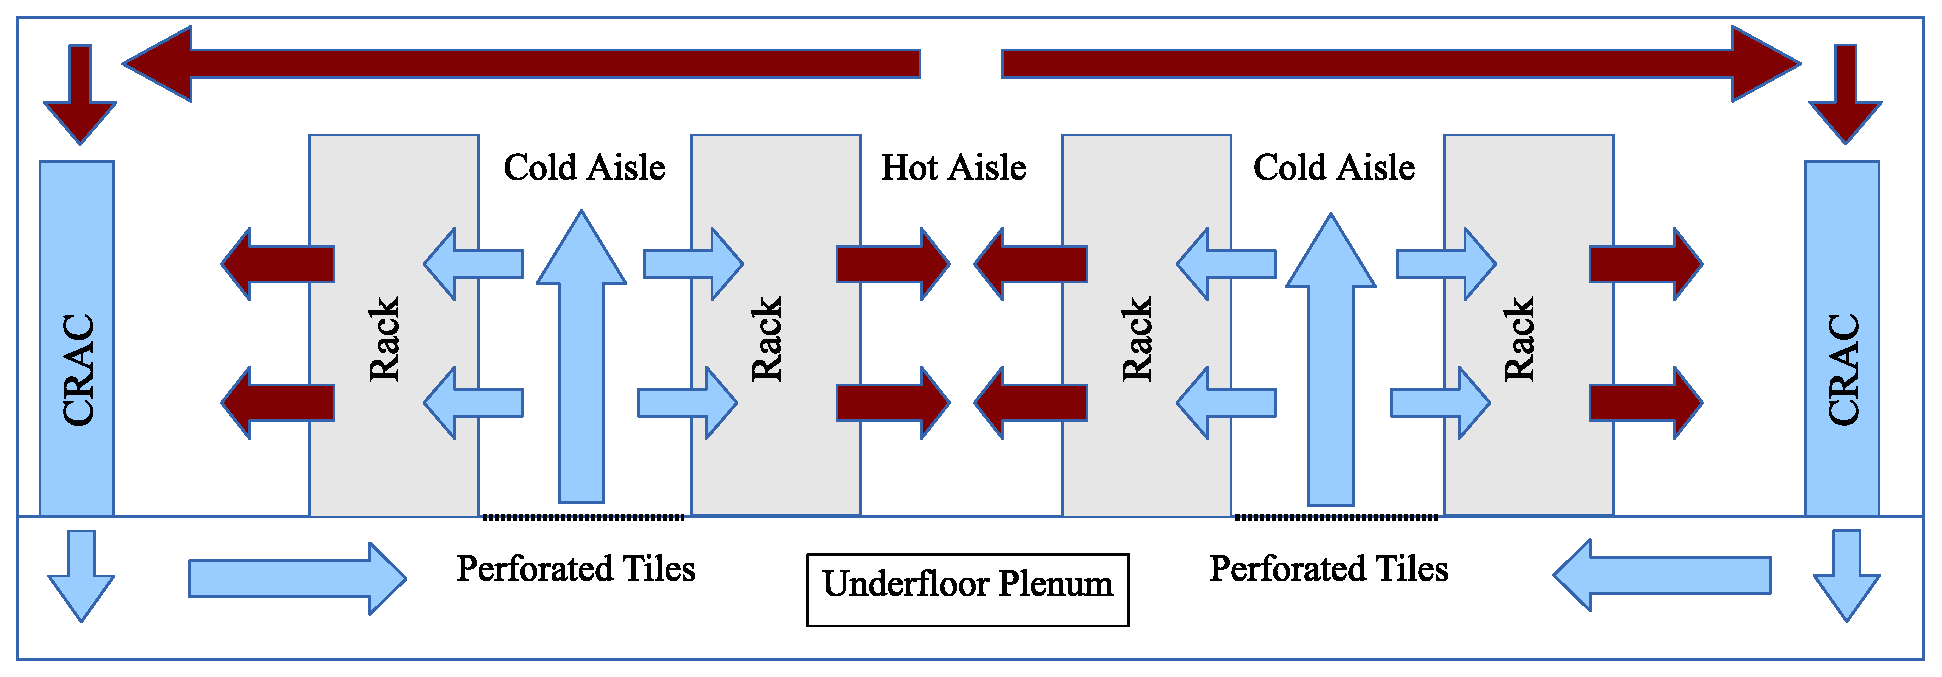
\includegraphics[width=\linewidth]{figs/DC_air_flow_tall}
\caption{DC air flow diagram showing the positioning of the racks, CRAC units,
underfloor supply plenum, perforated tiles, and the directions of the hot and
cold air streams. Side view.}
\label{fig:DC_air_flow}
\end{figure}

Data centers are deceptively simple installations when looking at the
essentials of making one. For our purposes, a DC is defined as ``any space
whose main function is to house servers''~\cite{Koomey2008}. First, as the
amount of computer servers increases, they are stacked to save floor space.
Then, the servers are installed into an external chassis called a rack. Racks
permit DC operators to remove a server for maintenance from the middle of the
stack without shutting down the other servers. The amount of servers in a rack
depends on both the server type and the rack height. When the rack is full, a
new one is brought in, and more servers can be installed into it.

Space permitting, multiple racks are installed side-by-side forming a row. As
the servers' air intakes are in their front, the idea is to keep each rack in
the row facing the same direction. This limits the hot exhaust air from mixing
with the cold intake air. Row length is dictated by floor space and ease of
maintenance, as cable connections are normally in the servers' rear sections.
When a row is full, racks are installed in a new row. Now, a simple
optimization is to position the new row face-to-face with the first one, so
that their air intakes are opposite. This way, the new row's air intakes can
be provided fresh supply air, and not the exhaust of the first row. These two
rows form an \emph{aisle} between them, called the cold
aisle~\cite{Sullivan2000} due to the influx of supply air. When the third row
is added, it is positioned so that its exhausts are opposite to either the
first or the second row's exhausts. The newly formed exhaust aisle is then
called a hot aisle.

In order to maintain a stable temperature in the DC, exhaust air must
eventually be reconditioned. This task is handled by the cooling units, which
draw in exhaust air, cool it down, and blow it back into the DC as supply air.
Figure~\ref{fig:DC_air_flow} shows one example of computer room air
conditioning (CRAC) positioning, where the units are placed on the same floor
as the server racks. Here, the CRACs supply cool air by blowing it under a
raised floor, maintaining an overpressure in the so-called underfloor plenum.
The raised floor is built with removable tiles; in the cold aisle, the tiles
are replaced with perforated ones so that supply air is pushed upwards towards
the server intakes. But note that this example can not be generalized to all
DCs. CRACs may alternatively be positioned in the DC ceiling, a second floor
above the DC, or in-row with the racks themselves. These alternative
placements have the benefit that they do not require a raised floor, which can
be costly to install retroactively. The discussion on exactly which placement
is the most effective has been going on since at least 1991~\cite{Nakao1991}.
Though the solution depicted in Fig.~\ref{fig:DC_air_flow} has so far remained
conventional~\cite{Bailey2006,Niemann2010,Rasmussen2010}, at least some
high-efficiency DCs use two-floor placements~\cite{Hamilton2011,Miller2013}.

At this point a distinction\footnote{This distinction was originally lost in
translation while writing Pub.~\ref{pub:cac}, as the Finnish word
\emph{vakioilmastointikone} can be taken to mean either type of cooling
unit.} should be made between air conditioning (CRAC) and air handling (CRAH)
units. Formally, a CRAC uses an internal direct expansion (DX) compressor to
produce the required cooling, while a CRAH employs an external source for
cooling fluid.  This implies that CRACs are more self-contained, and require
only a supply of power to operate.  Connecting the external cooling source for
CRAHs is much more complex. This can consist of separate cooling fluid loops
to one or more central cooling plants, and onwards to further heat rejection
units located outside of the DC buildings. The reward for this added
complexity is a higher energy efficiency, as a central cooling plant can be
made more efficient than smaller distributed units. In common parlance the
terms CRAC \& CRAH have become quite mingled, with CRAC becoming more popular
due to its resemblance to consumer-grade air conditioning (AC) units.  Though
imprecise, we follow the general trend and use the term CRAC for all units. In
almost all cases of Sect.~\ref{sec:flagships}, the facilities employ CRAH
units, whereas the small-scale facilities described in Sect.~\ref{sec:closets}
typically employ CRACs.

Precisely where and how the cooling is produced becomes quite important from
the efficiency point of view. It is a key design decision when building DCs,
difficult to modify afterwards, and can depend on the location of the DC.
Similarly, how exhaust air is removed and recycled, and how air streams are
separated are active research topics. We will return to these problems in
Sect.~\ref{sec:flagships}, as we review some of the state of the art
installations and what is known and unknown about them. In
Ch.~\ref{ch:retrofits} we will describe the main contributions of this thesis:
a set of low cost retrofit techniques that are very attractive to the larger
part of DCs worldwide.

What falls outside of the scope of this thesis are the
network~\cite{Kant2009,Abts2012} and power topology designs of the DCs. Very
briefly, network and power connections are installed per rack, meaning that
each new rack has an associated starting cost. The costs and available network
bandwidth limit the distribution of the servers in the racks. Therefore, it is
beneficial for a DC operator to try to keep the racks full before starting a
new rack. Likewise, sets of servers installed at approximately the same time
can be positioned close to each other to enable high-bandwidth data
interconnections or just to form logical maintenance units. Taken together,
these two facts mean that, for example, all of the servers of a
high-performance computing cluster are installed side-by-side. As higher
performance has so far meant a higher power draw, these points with higher
power intensities can form exhaust
hotspots~\cite{Bailey2006,Woods2010,Google2011,Seymour2011}. The hotspots then
dictate the requirements for the DC's cooling system. If servers are purchased
iteratively, e.g., by following periodic budget constraints, this type of DC
\emph{evolution} yields a heterogeneous mix of server generations and power
intensities throughout the DC.  

Conversely, it is possible for a DC to remain somewhat homogeneous, if the
servers are purchased approximately simultaneously, or if the DC operators
assemble their server hardware themselves. This type of DC operation has been
aptly named warehouse-scale computing by Barroso and
Hölzle~\cite{Barroso2009}, although the idea of treating the DC as a computer
was already mentioned by Patel et al. in 2001~\cite{Patel2001}. The general
idea is to redirect traffic between different DCs based on service
availability, congestion, and client request patterns. Consequently, this mode
of operation is possible only for those operators with multiple DCs at their
disposal. Natural catastrophes and unlikely failure mechanisms can and do
bring down entire DCs~\cite{Christian2012}, making redundancy a requirement
even at this level. But redundancy can become at odds with efficiency.


\section{Efficiency Metrics}
\label{sec:metrics}

By far the best-known metric for general DC energy efficiency is the power
usage efficiency (PUE) number defined by The Green Grid (TGG) non-profit
consortium~\cite{Azevedo2011,Belady2008a}. PUE is calculated very elegantly as
follows.

$$ \text{PUE} = \frac{\text{Total facility load}}{\text{IT equipment load}} $$

Total facility load is measured at the DC's power distribution grid
connection, and then divided by the aggregate power draw of all of the
computing servers. For long-term measurements, PUE can also be measured by the
energy used~\cite{Haas2009}. Special care must be taken while counting only
the hardware that belongs to the IT equipment load~\cite{Belady2008a}. For
example, power conversion losses caused by the servers' power supply units
(PSUs) are part of the IT equipment load, whereas all other conversion losses
related to cabling, voltage transformations, uninterruptible power source
(UPS) battery conversions, etc., are not. Similarly, fans inside of the
servers are counted as a part of the IT equipment load, whereas CRAC fans are
not.

PUE has no upper bound, and in practice, the facility load should always be a
little bit above the IT equipment load. A smaller PUE indicates a more
effective facility. The minimum was later clarified to be 1.0, meaning that
clever tricks like heat reuse can not turn the facility overhead into
negative. For heat reuse there is a different metric, the energy reuse
efficiency (ERE)~\cite{Azevedo2011,Patterson2010}, though DCs employing reuse
are still few.

PUE is ingenious in that it obfuscates both the size and capital expenses of
the DC, and thus concentrates on the operational expenses alone.  This allows
both operators to maintain secrecy about their design choices, and making
comparisons between vastly different types of DCs, though the latter has been
discouraged~\cite{Haas2009}. Unfortunately, verifiable information on what
represents good, average, or bad PUE numbers is somewhat lacking. Some IT
companies like Google~\cite{Google2013} and Facebook~\cite{McTiernan2013} do
publish their own PUE numbers, but the calculations are not reviewed
independently. According to their own info, Google's average PUE over their
entire DC fleet is 1.1 as of Q2/2013, with some facilities below 1.06. By
comparison, Facebook currently publishes the PUE readings from two of their
sites, showcasing an annual PUE of 1.09 as of March 2013 for the Prineville
site and 1.10 as of Q1/2013 for Forest City. The average for all DCs was 1.09
for 2012~\cite{Facebook2013}.

Other sources for PUE data include The Uptime Institute's survey from
March-April 2012~\cite{Stansberry2012} and EPA's DC report from
2010~\cite{Sullivan2010}. Uptime's survey includes over 1100 DC end users from
all over the world, and they report an average PUE value between 1.8 and 1.89.
Note that respondents were asked to select a category for the average PUE of
their largest DC only, 75\% ran more than one DC, and 29\% responded that they
do not collect PUE at all. EPA's report presents an average PUE of 1.91 from a
study of 108 DCs\footnote{There is some confusion in the available sources
regarding how many DCs EPA averaged over. Their model is composed of 61 DCs,
but the histogram on slide 20 of~\cite{Sullivan2010} adds up to 108.  This
number is also mentioned on slide 18.}. EPA's DC operators have supplied their
data voluntarily, which has lead to some suspicion that the results might
overestimate those DCs with favorable PUEs to begin with~\cite{Koomey2011}.
While it is clear that the sample is not statistically representative for all
DCs, it seems unlikely that the measured DCs were very optimized. EPA's
presentation of the data demonstrates that neither the top 10 DCs operating in
the coldest or warmest climates showed any variability in their monthly energy
consumption.

A lack of variance by climate is indicative of closed-loop cooling system, as
the main method of achieving a low PUE number is by different \emph{economizer
modes}, in which the cooling system uses less electricity but may consume
other resources. The straightforward way to achieve this is to employ local
reservoirs of cold air, water, or both~\cite{Niemann2010}. These reservoirs
are thus climate-dependent. Their availability is the reason why a DC's
location becomes so important~\cite{Gilder2006,Woods2010}, though a tradeoff
exists between the coldest possible locations and the available network and
power supply connections to them.

The use of tap water can achieve low-energy cooling even if no local sources
are available. This has lead to some DCs becoming increasingly
energy-efficient at the cost of wasting potable water. A separate metric, the
water usage effectiveness (WUE) has been proposed by TGG~\cite{Patterson2011},
but WUE has not yet achieved similar success as PUE. The situation is
improving, however, as 34\% of Uptime's~\cite{Stansberry2012} responders are
already collecting water usage data. Sharma et al.~\cite{Sharma2009} noted
that the matter of using water is even more complex, as water is also consumed
indirectly by the power generation processes. Thus, local water used at the DC
site may reduce the water consumed by the power utility. The problem with the
efficiency metric proposed by Sharma et al. is that it requires calculating
the water used indirectly in the generation of power. In some countries, like
Finland, Norway, Sweden, Denmark, and Estonia, power is generated by a mixture
of different generation facilities, and may be transmitted through the power
utilities' interconnects over the country borders~\cite{Entso-E2013}. Fingrid,
who operates the Finnish part of the grid, quotes transmission losses of 1.8\%
over a transfer volume of 64.2~TWh in 2012~\cite{Fingrid2012}. This means that
DCs connected to modern transmission grids are not bound to using only locally
generated electricity, e.g., coal, but may purchase it over longer distances.


\section{Flagship Facilities}
\label{sec:flagships}

Location has become a key driver for DC placement in multiple ways. DCs
operating in the U.S., have been repeatedly criticized for their placement in
rural regions that yield cheap floor space, but are also powered by
traditional coal-based power plants~\cite{Huber1999,VanHorn2011}, or even
their own diesel-powered generators~\cite{Glantz2012b}. Later, the trend has
reversed so that DC placement has favored locations close to hydroelectric
dams~\cite{Gilder2006}, keeping the logic that the DC is powered by the
closest facility only. But when the electricity is generated by a mix of
strategies following shifts in demand and supply, those generators that can
ramp production up or down are typically coal- or gas-based installations.
This means that green energy sources are always used to their full capacity,
and without the DC there would simply be other consumers for the renewable
energy.
% FIXME: invent a source for the above idea

Fortunately, the situation can be circumvented. If DC operators make
commitments ensuring that \emph{more} renewable energy sources get installed,
the additional supply will follow the increased demand of DCs. This is the
style of operation for Google, which has repeatedly purchased sources for
renewable
energy\footnote{\url{http://www.google.com/green/energy/investments/}} to make
up for the demand of its DC fleet. One such notable example is the case of
Google's Hamina site, located on the southern coast of Finland. Here, the DC
has committed to purchasing all the energy produced by a wind farm in
Maevaara, northern Sweden~\cite{Sterin2013}, over a distance of ca. 680~km.
The Hamina site is also notable for being the only one of Google's DCs to use
sea water as its only cooling source~\cite{Larsson2010,Metz2010,Metz2012}.
Another notable Google DC is the one in Saint-Ghislain, Belgium, which
reportedly began operation without chillers all-year~\cite{Miller2009}. The
site has later added a water purification facility that collects water from
the nearby Nimy Blaton canal, and purifies the water to make it usable for
cooling purposes~\cite{Miller2010,Metz2012}. Other Google water collection
schemes involve reclaiming graywater from a municipality near their DC in
Douglas County, Georgia, U.S.~\cite{Brown2012} and rainwater collection on an
undisclosed site\footnote{Probably Berkeley County, South Carolina according
to
\url{http://www.google.com/about/datacenters/inside/locations/berkeley-county/index.html}.}
in the U.S.~\cite{Miller2010}.

Around year 2011, Facebook became the prime target for Greenpeace's campaign
for DCs to ``unfriend dirty coal''~\cite{VanHorn2011}. Facebook was quick to
adapt, however, and has since increased its dependence on renewable energy
sources~\cite{Meikle2011}. As a follow-up, Facebook has become one of the most
transparent companies when it comes to the energy-efficiency of its DCs.  Not
only does the company report near real-time PUEs~\cite{McTiernan2013}, but
also WUEs and total power draws for its DCs~\cite{Facebook2013}. Facebook is
also one of the principal operators behind the Open Compute
Project\footnote{\url{http://www.opencompute.org/}}, which aims to publish new
and more energy-efficient designs for DC operation. As a result, Facebook's
Prineville (Oregon, U.S.) site's cooling design is exceptionally well
documented by Hamilton~\cite{Hamilton2011}. Hamilton is also the vice
president of the Amazon Web Services team, making Prineville perhaps the first
publicly peer-reviewed DC in the world. The facility employs ``air conditioner
bypass via direct air with evaporative assist'' by Niemann's
classification~\cite{Niemann2010}, meaning that the DC draws in outside air
and if necessary, conditions it with an evaporative system to a temperature
suitable for cooling. This cooling technique is also known as adiabatic
cooling. The exhaust air is drawn to a second floor above the racks, from
where the air may be reused to warm supply air if the ambient temperature
drops too low~\cite{Hamilton2011}. Despite its successful design, the exhaust
loop did cause a sizeable number of problems when a malfunction in the
circulation logic caused the exhaust to be entirely recirculated. As the
humidity levels started increasing, condensation occurred inside the DC,
killing a number of power supplies and other components~\cite{Mulay2011}.
These problems were fixed, however, and Facebook duplicated the Prineville
design in its DC based in Luleå, northern Sweden.

The Luleå site is famous for being located in the intersection of multiple
power supply lines originating from several hydroelectric dams in the
vicinity. The overlapping supply feeds have enabled Facebook to avoid backup
power up to 70\% of their normal standards~\cite{Miller2011,Miller2013}. This
event signals a very important shift in the design logic of DCs, namely that
of depending \emph{more} on the state- or municipality-provided infrastructure
instead of duplicating it for redundancy. A similar dependence has been seen
earlier in the case of formerly Academica's, now TelecityGroup's DCs in
Helsinki, Finland. Their facilities have been award-winning in their
efficiency thanks to the contribution of the district cooling grid run by the
capitol's energy utility, Helsingin Energia~\cite{Uptime2010}. This district
cooling grid was initially built around year 2000, and it complements the much
wider district heating grid of the city constructed around 1953--1957. The
cooling grid employs seawater as a natural cold reservoir which is used to
cool down facilities connected to the district cooling grid.  Examples include
hospitals, but also office air conditioning systems. As the cool water gets
heated up in the process, this energy may later be extracted by the utility
and then used to warm the district heating grid.

Another marine source for cooling is the North Sea, or at least the winds
cooled by it. HP's Wynyard DC site is located near Dublin, Ireland. Its
original web site has disappeared from the company's servers, but the contents
are still available thanks to the Internet Archive~\cite{HP2009}. Wynyard is
notable for incorporating an early (2009) direct air economizer that draws in
the naturally cold sea winds. The cooling setup is also remarkably similar to
Facebook's Prineville, with the exception of using CAC (see
Pub.~\ref{pub:cac}) instead of hot aisle containment
(HAC)~\cite{Hamilton2011}. As a consequence, Wynyard claimed a PUE of 1.16
already in 2010~\cite{Saran2010}.

Microsoft also began operating a DC \emph{almost} without chillers near Dublin
in 2009~\cite{Metz2009}. Originally, the facility operated with backup DX
chillers for those periods each year the ambient temperature might exceed
35$^\circ$~C. This supply temperature is somewhat of a maximum for a
large-scale DC, as several PC manufacturers cite it as the upper endpoint of
the operating range~\cite{Belady2008,Google2011}. The original PUE was
announced as 1.25~\cite{Microsoft2009}, but has later been improved by
replacing the backup DX chillers with an adiabatic cooling
system~\cite{Miller2013b}. This and possibly other improvements have reduced
the PUE to 1.17. Microsoft's Dublin DC seems to both supply intake and remove
exhaust air through the roof of the facility.

Affectionately known as the ``chicken coop DC''~\cite{Miller2010b}, Yahoo's
Computing Coop (YCC) solution is different from earlier DC designs. In this
case the entire building is left as open to the ambient temperature as
possible, and hot air is gathered by a protrusion on the roof. The maximal use
of outside air used is reported to result in only 212 hours per year when
extra cooling is required. The YCC was originally completed in 2010. The same
year, Microsoft announced a similar design nicknamed the ``tractor
shed''~\cite{Miller2011}. The concepts are similar, but the servers in the
shed are further housed in Microsoft's IT Pre-Assembled Components (IT PACs),
which are modular containers that include the necessary network interconnects,
power supply and -backup units. Modular containers have slowly become more
widespread~\cite{Stansberry2012}, but Quincy is the largest DC using them that
we know of.

Finally, it is interesting to note a few similarities between these DCs. Upon
its announcement, Microsoft's Dublin site was reported as a replication of
Google's Saint-Ghislain DC~\cite{Metz2009}. Yahoo's Lockport and Microsoft's
Quincy certainly share similarities, although Microsoft's solution is further
divided into the IT PAC modules. The air flow schematics of HP's
Wynyard~\cite{Saran2010} and Facebook's Prineville~\cite{Hamilton2011} are
remarkably alike, although with the difference of using CAC vs. HAC. It would
be easy to attribute these similarities to individual workers switching camps,
but they may also result from the convergence of the R\&D processes.  Whatever
the cause, it is safe to say that the largest and most efficient DCs do
resemble each other. But they do not resemble smaller DCs.



\section{Different Types of Data Centers}
\label{sec:types}

In 2012, a popular article published in The New York Times concentrated on the
sustainability of many DCs by drawing focus on their high energy
requirements~\cite{Glantz2012}. By itself, the story had novelty mainly for
the general public, as the situation was already well known to both academics
and the industry. Other factions, e.g., Greenpeace, were already known for
having taken potshots toward individual DC operators like
Facebook~\cite{Meikle2011,VanHorn2011}.  In 1999, a somewhat sensationalist
piece published by Forbes~\cite{Huber1999} had raised an early
controversy~\cite{EPA2007} by suggesting that before 2010, half of all
energy consumed in the U.S. would be consumed by DCs.

What was notable about the 2012 article was the author's long-term background
research, including a sizeable number of interviews with DC operators and
other experts. The diligent study allowed J.~Glantz to paint a reasonably
complete picture of the operation of different DCs. Despite its merits, many
expert readers felt that the article had omitted a vital aspect of DCs: that
there is not a single type of data center, but
several~\cite{Koomey2012a,Petersen2012,Woods2012}. The importance of the
division forms around the fact that the different types of DCs are maintained
very differently. Most notably, the very largest DCs, which consume the most
energy, are typically operated much more meticulously than smaller facilities.

In his response to the New York Times' article, Koomey formalized this
classification and coined the four subtypes of DCs~\cite{Koomey2012}. This
categorization is of particular importance as it reflects well with the
earlier grouping of DCs into small, medium, and large-scale facilities used by
the International Data Consortium (IDC) in
2007~\cite{Bailey2006,Bramfitt2012}. We will return to their relative sizes in
the beginning of Sect.~\ref{sec:closets}, but first describe the DC
categories.

The first type of DC is the best known, for this type includes many of the
so-called flagship installations operated by the IT industry giants, e.g.,
``Amazon, Google, Facebook, and Microsoft''. Section~\ref{sec:flagships} adds
instances operated by Yahoo and HP into this category. These DCs are usually
showcased by large ICT companies in order to prove their relative
``greenness'' and dedication to sustainable operation. And there is some truth
in this, for the public cloud computing providers do excel in the energy
efficiency of their facilities, since their business models depend on this.
But note that this relationship is strictly one-way: not all of the DCs
operated by a cloud providers are equally efficient. They also run much
smaller facilities~\cite{Google2011} that fit better into the other
categories.

Second, the scientific computing centers are distinct for their user request
patterns. While it can be argued that most of the cloud is dependent on the
online services accessed by the clients at the network edge, scientific
facilities often specialize in high-performance computing only. This means
that their processing tasks may resemble much more the venerable
batch-processing operating systems of yesterday. Hence, scientific facilities
can show much more impressive utilization ratios. For example, National Energy
Research Scientific Computing Center showcased an utilization ratio of 96.4\%
during July 2012~\cite{Glantz2012}.

Colocation (colo) facilities are run by vendors who, like the cloud providers,
specialize in running DCs. The difference is that the colo operators expertise
cover only the placement, construction, operation, and maintenance of the DC
infrastructure. The specific IT hardware installed can be provided or
recommended by the colo contract, sometimes called a ``hosting'' contract, or
left entirely as the customer's choice, indicating a ``housing'' version.
Colocation can be very good for online services that further depend on other
services, e.g., online trading~\cite{Glantz2013}. This results in companies
paying quite high premiums for some colo facilities depending on their
physical location and network connection characteristics. Beyond cultivating
these types of relationships, what falls outside of the colo operators' domain
are the applications that run inside the DC. This means that the average
server utilizations can be much lower than in the case of the public cloud's,
and on par with the last category of DCs.

The last category was tentatively named the ``in-house'' DCs by Koomey. This
title reflects upon the primary mode of operation for the companies housing
these DCs, which tends to be other than computing. In-house DCs are usually
office or technical spaces converted for DC use, and contain servers which
have been stepwise acquired as needed by other company processes. It is this
category which tends to contain the smallest facilities, involve the most
wasteful practices, and be the largest of the four by numbers.


\section{Server Closets}
\label{sec:closets}

\begin{table}
  \centering
  \begin{tabular}{l|r|r|r|r} \hline
 & \# servers & PUE & avg \# servers & total energy \\
 \hline
Server closet & 1,657,947 & 1 & 1 & 11\% \\
Server room & 1,942,214 & 1.9 & 2 & 24\% \\
Localized DC & 1,674,648 & 1.9 & 26 & 21\% \\
Mid-Tier DC & 1,511,999 & 1.9 & 161 & 19\% \\
Enterprise-class DC & 3,074,424 & 1.2 & 491 & 24\% \\
 \hline
Total & 9,863,237 & & & 100\% \\
  \end{tabular}
  \caption{Power consumed by the combined servers of different categories of
  DCs. Calculated as number of servers $\times$ watts per server $\times$ PUE.
  Percentages shown are fractions of the sum of power consumed by all DCs.
  Numbers from IDC's 2006 report~\cite{Bailey2006}.}
  \label{tab:closets}
\end{table}

During the 2011 European Data Centre Summit hosted by Google, the keynote
speech by U. Hölzle~\cite{Holzle2011} contained a very concrete message for
the researchers and engineers present: concentrate on improving the
non-enterprise DC facilities. By drawing upon the data published in 2006 by
the IDC~\cite{Bailey2006}, and further analyzed by the National Resources
Defense Council (NRDC)~\cite{Bramfitt2012}\footnote{Citation refers to the
2012 version of the report, earlier versions contained the same division of
DCs.}, Hölzle presented an easily digestible infographic that divided the
installed server base at the network core into categories based on the sizes
of the DC facilities. Hölzle's simplified version showed the installed servers
to be split up into 41\% ``closet \& small'', 31\% ``localized \& medium'',
and 28\% ``enterprise'' DCs~\cite{Holzle2011,Bramfitt2012}. The actual data
from IDC is somewhat more granular\footnote{There is a discrepancy between the
percentages reported by NRDC~\cite{Bramfitt2012} and the absolute numbers from
IDC~\cite{Bailey2006}. Our percentages are calculated from IDC's numbers.},
further dividing the smallest category into 17\% of size ``server closet'' and
20\% ``server room'', and the middle category into 17\% ``localized'' and 15\%
``mid-tier''.  Last, ``enterprise-class'' makes up for the remaining 31\%. The
size limits defined for the categories are, in increasing order, less than 200
ft$^2$ ($<$19~m$^2$), less than 500~ft$^2$ ($<$47~m$^2$), less than 1,000
ft$^2$ ($<$93~m$^2$), less than 5,000 ft$^2$ ($<$465~m$^2$), and over 5,000
ft$^2$~\cite{Bailey2006,Bramfitt2012}.

The vast majority of the DCs belong to the two smallest categories. According
to IDC~\cite{Bailey2006}, a full 51\% of all DCs belong to the smallest
category of server closets, with an additional 45.5\% in the next-smallest
category of server rooms. Taken together, these two categories numbered about
2.2 million in 2005, compared with the just under 80,000 of all other DCs.
What's worse, between 2005-2009 the two smallest categories were projected to
increase with compound annual growth rates (CAGR) of 4\% and 3.3\%,
respectively, compared with the CAGRs of 0.0\%, 1.0\%, and 2.8\% of the larger
categories (ordered by DC size).

While the IDC report could not tell much about the amounts of power the
different DCs were using, by looking at the PUEs of the enterprise-class DCs
presented in Sect.~\ref{sec:flagships} and the average PUEs described by the
surveys discussed in Sect.~\ref{sec:metrics}, we can make some conservative
estimates. It seems that by now, the ICT industry giants all know how to build
a DC with a PUE of 1.2 or less, so we will use that as an estimate for the
enterprise-class DCs. Currently documented average PUEs are close to 1.9, and
were reported for the largest DC of operators with at least (75\%) one
facility~\cite{Stansberry2012}. Thus, we will use this number for the
localized and mid-tier categories. Next, IDC's DC taxonomy~\cite{Bailey2006}
describes the smallest category of server closets as usually not containing
cooling or backup power systems. Hence, we use a PUE of 1.0 for these DCs, as
the requirements for power conversion and lighting are negligible when, on
average, only a single server is installed. Finally, it is very difficult to
estimate a PUE for the next-smallest category of server rooms.  IDC does
mention that these rooms have ``upgraded air conditioning, UPS equipment, and
some security''. Without further evidence, we have duplicated a PUE of 1.9 for
this category as well.

Table~\ref{tab:closets} plots the relative amounts of energy used by the
different DC categories based on the assumptions given above. By adjusting for
the power consumed by the whole DC based on the estimated PUE metrics of the
different categories, we can see that the smallest two categories draw a
little over a third of the combined power consumed by all DCs. The next two
categories account for an additional 40\%, with the largest, enterprise-class
DCs being responsible for the last 24\%. Thus, while the largest DCs should
manifest the newest and most energy-efficient, techniques, 76\% of the power
is drawn elsewhere. There are at least two alternatives that may be attempted
to reduce the aggregate power draw of the combined non-enterprise DCs. 

The first is to implement techniques that can be incorporated cost-effectively
and quickly by the operators of the non-enterprise DCs. In the next chapter,
we will introduce the main contribution of the thesis, techniques which fit
this description of \emph{data center energy retrofits}. Sadly, not all
techniques can be applied in all cases.  IDC's report also outlines the
average number of servers in each category, and while the two smallest
categories dominate the number of DCs, they may contain as few as one or two
servers per DC on average. This makes it plausible that some of our techniques
are most useful for the middle categories. However, while these are averages,
individual installations do vary. In Sect.~\ref{sec:discussion} we will
revisit the applicability of our techniques per DC category.

The second alternative involves migrating all services to larger and more
efficient DCs, and then shutting down the smaller installations. The second
alternative has so far proven difficult, as not only the operating costs
involved, but also laws and regulations have hindered some DC operators from
shifting their confidential data across country borders to the
cloud~\cite{Bailey2006,Gallagher2013}. And this may have been a good thing.




% Chapter
\chapter{Energy Retrofits}
\label{ch:retrofits}

The history of computation suggests that there have been several
back-and-forth movements of where the larger part of data processing is
performed. The earliest change occurred when most users stopped working on
university-scale computing machinery and turned instead to personal computers.
These distribution shifts manifest as differing distances a user request has
to travel before its response is formed. For example, current mobile clients
can offload tasks to networked servers in order to save local battery
lifetimes.  Thus, we are still experiencing a shift towards the core of the
network. As mentioned in Sect.~\ref{sec:types}, there have been attempts to
criticize this shift by questioning the energy demands of the
DCs~\cite{Huber1999,VanHorn2011}. So far, the attempts have not thwarted the
growth of the industry. This situation might now be changing, since the new
issue brought to public consciousness concerns the \emph{trust} users put into
the DC operators, and whether that trust has been misplaced.

Edward Snowden is the whistleblower who quickly rose to public prominence
during June 2013~\cite{Greenwald2013,Gellman2013}. In his iconic,
closely-cropped video interviews, Snowden explained his background as an
employee of a company subcontracted by the National Security Agency (NSA). It
had been part of Snowden's job as an analyst to mine the databases the NSA had
at its disposal for signs of international terrorism.  Snowden explained that
the job included not only the capability, but a routine to tap into several
DC operators' databases, including ``Google, Facebook, Apple, Microsoft''.

Later articles have verified Snowden's story and expanded on the abilities of
the so called XKeyscore interface, one of the tools NSA has at its
disposal~\cite{Greenwald2013a}. At the time of writing, the jury is still
literally out to decide whether NSA will keep its monitoring
privileges~\cite{Sirer2013}. Regardless of the verdict, considerable damage
has already been done to the DC operators who were forced to participate in
the program by a combination of U.S. laws and gag orders~\cite{Gallagher2013}.
The latter have been especially harmful, for they still prevent DC operators
from revealing the true extent of the monitoring~\cite{Drummond2013}. While
earlier articles have presented facts about the energy efficiency, or lack
thereof, of the DC industry, the new situation is different for it plays on
the users' \emph{fears} of the unknown due to the gag orders.

It is an open question whether the aftermath will trigger IT operators to
re-embrace their server closets.  Very generally, there are two options for
the future\footnote{There is a third option as well. The occurrence of a so
called \emph{disruptive event} could cause the public to hasten the migration
to the public cloud, despite the continuing surveillance of the government
agencies.}. First, if the public outbreak tones down, and the migration of the
closets to the high-efficiency cloud and colo DCs continues unabated, this
chapter's techniques will remain usable for the immediate future. As the
payback times are in all cases very short, even a delay of a few years will
yield savings. And since national and regional data storage laws have thus far
prevented the migration altogether in some
cases~\cite{Bailey2006,Gallagher2013}, some server closets might remain in
operation for the foreseeable future. The second alternative is much worse for
the energy efficiency. If the users decide that the cloud may no longer be
trusted, a distribution shift back towards the network edge might occur. In
this case the efficiencies of the server closets will grow more important. We
will need not only cooling solutions, but a wide range of energy improvements
that can be adapted all the way down to the very smallest DCs.

We are not the only ones who have recognized the problem of optimizing the
non-enterprise DCs. In the 2011 European DC Summit mentioned in
Sect.~\ref{sec:closets}, Google introduced their own small-scale optimization
study. The video feature, web site, and accompanying white paper outlined the
steps Google had taken along with the PUE improvements
achieved~\cite{Google2011}.  While looking at the presentation I confess to
having felt a certain degree of accomplishment, for Pub.~\ref{pub:cac} had
already been submitted, and the air stream containment we had built differed
from Google's solution mainly by the materials used. While our solutions were
not yet polished to the same presentational levels, the core ideas were
similar. Neither we nor Google stopped there, however. The three best
practices introduced by their study involved a 85~kW DC that was stepwise
improved from a PUE of 2.4 to a much more impressive 1.5. The same changes
were later reproduced in four other DCs. The best practices were as follows:

\begin{enumerate}
  \item{Measure performance}
  \item{Optimize air flow}
  \item{Turn up the thermostat}
\end{enumerate}

There are quite direct connections between these best practices and four of
our publications, although the order in which we experimented was somewhat
different than Google's. Publication~\ref{pub:zero} was done first, and it
involved turning the thermostat up, or in our case, down. It will be presented
in Sect.~\ref{sec:free}.  Publications~\ref{pub:cac} and \ref{pub:uac} detail
our implementation of CAC and its extension, underfloor air containment (UAC).
These solutions are detailed in Sect.~\ref{sec:air}. Next,
Pub.~\ref{pub:greenhouse} presented in Sect.~\ref{sec:harvesting} falls
outside the best practices of Google, and paves the way for future work, in
which we hope to see DCs that direct their waste heat for useful purposes.
Finally, while Pub.~\ref{pub:sensors} is directly related with the category of
measuring performance, it has significant differences to Google's approach of
using CFD. Because of this, we describe the wired sensor network in
Sect.~\ref{sec:costs}, which covers the different strengths and weaknesses of
building actual prototypes vs. CFD-based modelling studies.


\section{Free Cooling}
\label{sec:free}

As outlined in Sect.~\ref{sec:metrics}, one of the straight-forward methods of
improving PUE is to employ a cooling system that has an economizer mode.
Another option is to increase the supply temperature of the CRACs, which
reduces the power used for cooling, but also warms the air which reaches the
server intakes. The limits set on how high the intake temperature may reach
have traditionally been made by two authorities: the server manufacturers'
warranties and the American Society of Heating, Refrigerating and
Air-Conditioning Engineers, Inc.'s (ASHRAE) recommendations. The problem with
both sources is their bias in reporting operating temperatures lower than
necessary for the server equipment~\cite{Moss2011}. In the case of the server
manufacturers, this mode of operation is known as
sandbagging~\cite{Belady2008}, and it is done in order to insure that the
equipment reliability is not compromised. The members of ASHRAE are vendors of
cooling equipment, and it would be quite disastrous for some of their business
if it was discovered that a properly located DC requires no cooling
whatsoever.

Such a discovery was anticipated by McKeown already in 1986~\cite{McKeown1986}
and finally presented by both Intel~\cite{Atwood2008} and
Microsoft~\cite{Belady2008} in 2008. Both companies published proof-of-concept
(POC) reports of installations where servers had been air cooled using direct
outside air. Intel's experiment involved running 896 blade servers for ten
months divided into two (2 $\times$ 448) compartments, one with a DX cooling
system using an air economizer and the other with a conventional CRAC.  No
humidity control was involved in either compartment.  The failure rates showed
a small increase from 2.45\% in the DX to 4.46\% in the economizer
compartment~\cite{Atwood2008}. While seemingly a significant elevation, no
rigorous statistical analysis was presented, so the elevation could also have
been caused by random variation. In the case of Microsoft, there are much
fewer details available~\cite{Belady2008}. The servers subjected to the test
amounted to five HP DL385 units running for 7--8 months with zero
failures. More interestingly, Microsoft ran the servers in a tent and
subjected them much more thoroughly to the mercy of the ambient climate.

While we were oblivious\footnote{We were unaware of Microsoft's experiment in
our review of related work for at the time, it was promoted by Microsoft with
much less enthusiasm than Intel and their POC.} of Microsoft's publication,
Intel's caught our interest. In Pub.~\ref{pub:zero} we describe our own
experiment, in which we installed 18(+1) servers pairwise indoors and in a
tent erected on the roof of the CS Dept. building. The servers in both groups
ran for a period of eight months, although Pub.~\ref{pub:zero} only contains
details for the first three months of operation\footnote{Two of the servers
have been reused in later experiments, and have thus far remained outdoors and
online for over \emph{three years} of operation. We are planning a follow-up
article.}. Our main research question was the feasibility of extending direct
free air cooling into the colder climate of Helsinki, Finland, and in the case
of a negative answer, what kind of new common-mode failures
(CMFs)~\cite{Avizienis2004} would appear in the very low local winter
temperatures.

When Pub.~\ref{pub:zero} was finished the answer to the feasibility question
was considered positive, for even at the end of the experiment and eight
months of operation, we had found no CMFs related to the temperature or
humidity ranges.  Since then, we have encountered a CMF related to one fan
type, and this failure mode is still under study~\cite{Pervila2013}. The
results of our research are important for air economizers seem to be abundant
in enterprise-class DCs. Whereas larger DCs can condition the outside air
using water and adiabatic systems, depending on the location, water supply
might be scarce. For smaller DCs the use of direct outside air would result in
the lowest capital expenses for the cooling solution. In addition, our
research complements other independent studies regarding the temperature
operating ranges of computer equipment, and how varying the temperatures
affects failure
rates~\cite{Elerath2004,Pinheiro2007,Schroeder2007,Schroeder2009,El-sayed2012}.
The newer analyses seem to question the previous ``industry folklore'' that a
lower operating temperature yields less failures. Many of the studies would
have remained impossible without data derived from warehouse-scale computing
architectures. The results are key in understanding whether the energy savings
of an elevated supply temperature are offset by an increase, if any, in
equipment replacement costs.

There may also exist upper bounds for the ambient temperatures at which
commercial, off-the-shelf (COTS) hardware should be
run~\cite{Malone2008,Patterson2008,Moss2010}. Due to the economies of scale
involved, it is financially prudent for DC operators to purchase large
quantities of so-called volume servers from the manufacturers. This implies
that the DC operators do not build their own servers, which is the approach of
at least some cloud operators, e.g., Google and Facebook. COTS servers contain
firmware controllers that set the operating speeds of internal fans according
to the ambient temperatures~\cite{Moss2010}. In addition but to a smaller
extent, leakage currents in components, including CPUs, are aggravated by
increases in the ambient temperature~\cite{Patterson2008}. A steadily
increasing supply temperature may thus yield savings at the CRAC, but
aggregate losses at the IT hardware level. As mentioned in the beginning of
Sect.~\ref{ch:state}, a heterogeneous mix of servers can cause hotspots where
the local temperature is elevated due to eddies in the air
flow~\cite{Moss2010}.  Therefore, optimizing the cooling in a DC involves not
only tuning the supply air temperatures, but also directing the air flow.



\section{Air Stream Containment}
\label{sec:air}

There are some reasons why direct outside air cooling might not be feasible
for all DCs despite a pre-selected and compatible climate. Mainly, particles
in the air~\cite{McKeown1986,Schmidt2002,Greenberg2006,Atwood2008,Belady2008}
from either pollution or plant-based pollen might be carried all the way into
the server intakes, and eventually cause fan failures~\cite{Pervila2013}.
Other reasons include external limitations on the DC location caused by laws
and regulations ~\cite{Bailey2006,Gallagher2013}, or the network latency
requirements of hosted web services~\cite{Glantz2013}. In-house DCs may also
be located so that no pathway exists for delivering outside air to the DC.

Even if the cooling is derived from direct outside air or an air economizer,
problems in the DC's \emph{internal} air flow may cause inefficiencies that
result in temperature hotspots.  Consider the example CRAC positioning of
Fig.~\ref{fig:DC_air_flow} where supply air is diverted through perforated
tiles upwards into the cold aisle, and conversely the exhaust air is pushed
into hot aisles by server fans.  Already in 1991, Nakao et
al.~\cite{Nakao1991} identified the effects of exhaust air short-circuiting,
i.e., mixing of the hot and cold air streams.  This phenomenon results in
wasted cooling capacity either through unnecessary warming of the intake air
or cooling leakages in the hot aisles.  The mixing may occur either around the
edges of the rack rows, or directly through them if there are gaps without
servers in the racks. An underpressure in the cold aisle side caused by an
insufficient ratio of CRAC supply to server intake
air~\cite{Germagian2009,Seymour2011}, may draw the exhaust around the racks,
or in some observable cases, even through servers with less powerful fans (see
Pub.~\ref{pub:sensors}). Similarly, if the CRAC units' return-side fans are
not operating at sufficient levels, an exhaust side overpressure may push the
exhaust back into the cold aisle.

In Pub.~\ref{pub:cac} we examine a by now very well-known technique used to
mitigate air stream mixing, cold aisle containment (CAC). With CAC, the cold
aisles are contained with side walls and roofs which separate the supply and
exhaust air flows. CAC was identified as a key optimization technique by
Google in 2011~\cite{Google2011}, and it has been documented in at least one
white paper by HP in 2009~\cite{Hilss2009}. Niemann mentioned home-brew CAC
setups already in 2008~\cite{Niemann2008}. In contrast to earlier works, ours
is the first scientific study that operates on a live DC. HP studied CAC
through emulating servers with load banks~\cite{Hilss2009} while we used a
real, heterogeneous and production-use 80~kW DC. We were able to perfectly
replicate HP's 20\% increase in blower air flow, which means that a DC using
CAC may install 20\% more servers while maintaining the same cooling solution.
More importantly, if CAC is installed to begin with, the DC may reduce the
CRACs' capital expenses. The key drawback of our study was that we were unable
to measure PUE changes due to the fact that our DC is connected to two
different chilling plants, with the second also used for other purposes.
Despite this, the 20\% reduction in supply air is expected to yield larger
savings in a holistic analysis, for the inefficiencies of the cooling system
mean that for a DC without CAC and a constant IT equipment load, the Total
facility load will be higher (see Sect.~\ref{sec:metrics}).

In Pub.~\ref{pub:uac} we revalidate our initial, homebrew DC CAC solution
built with duct tape and plastic sheets using a much more high quality, but
still DIY installation. The effects of the new CAC version remained identical
within our measurement errors, meaning that even a quick and dirty CAC just
works\footnote{Our YouTube presentation achieved over 40,000 views, raising
the public awareness towards this technique:
\url{http://www.youtube.com/watch?v=m8NcIN4rNqU}}. In the same publication, we
extend CAC to the underfloor plenum (see Fig.~\ref{fig:DC_air_flow}) and thus
direct the volume of supply air to more closely reach the server intakes.  Our
reason for working with the plenum was to study the effects of leakage air
flows caused by gaps in the raised floor tiles~\cite{Hannaford2006} and
underfloor blockages~\cite{VanGilder2005,Herrlin2006}, which are difficult to
study with CFD~\cite{Bhopte2006}. The construction materials are, again, as
cheap as possible. With an initial cost of just tens of euros, and an
installation time of just one hour for a 74~m$^2$ DC, we were able to measure
an additional 9\% improvement in the air speeds inside of the CAC. The new
solution was titled underfloor air containment (UAC). As CAC and UAC are
directly compatible in all DCs with an underfloor plenum, these techniques
complement not only each other, but also the free air cooling solution. For
even if the cooling is achieved for free, air blowers must still be used not
only to direct cold supply, but also for gathering warm exhaust air.



\section{Harvesting Heat}
\label{sec:harvesting}

Publication \ref{pub:cac} also introduced the Helsinki Chamber (HC), our
prototype chassis for direct outside air cooling. The concept of the HC
closely resembles ideas presented earlier by Church et al.~\cite{Church2008}
and Brenner et al.~\cite{Brenner,Brenner2009}. Church et al. presented the
unconventional idea of splitting a larger DC into multiple micro DCs that
would be located sparsely to avoid thermal hotspots. Brenner et al. start from
a different angle by placing their servers near a large greenhouse, which is
then heated by the exhaust air. Both lines of research involve distributing
the computation near the clients at the network edge. Our HC is the extension
of our earlier tent-based setup (Pub.~\ref{pub:zero}), but with dual chambers
for the cold and warm air streams. The HC has a PUE of exactly 1.0. By
combining the micro DCs with the CAC technique, we have successfully operated
servers for three years in the HC.

Our own greenhouse project started off from the endeavour to find some use for
a DC's waste heat. For this, we needed a realistic target to heat up.
Initial plans included building a sauna, but these were scrapped due to the
fact that we did not have engineering proficiency with the required heat
pumps. In the end we opted for a direct heat reuse target, and built a
lightweight greenhouse in connection to the HC. The main differences to
Brenner et al.~\cite{Brenner2009} are our edible crops and that the DC came
first, not the heating target.  Publication~\ref{pub:greenhouse} describes our
first eight months of operation and the edible plants we cultivated. At the
time of writing, we are well into the second growing season and batch of
plants. A number of volunteers have taken over and tend the plants, which
nowadays consist of chilies only.

For many reasons, growing chilies with the exhaust heat of servers has been
met with a spectacularly good media reception, and our project has been
mentioned in numerous blog posts, the social media, and the largest local
newspapers\footnote{We maintain a partial list at
\url{https://wiki.helsinki.fi/display/Exactum5D/Citations}}. This was not
entirely unexpected, as the experiment was designed with also the PR value in
mind. We did this in order to raise the public awareness about the waste heat
produced by many DCs, since currently most heat is just dumped into bodies of
air, water, or both~\cite{Hamilton2010}.

Some exceptions exist, though. One of the DCs presented in
Sect~\ref{sec:flagships}, the one by Academica /
TeleCityGroup~\cite{Uptime2010}, already falls into this category, and it
would be beneficial for the energy efficiency of the larger community if this
trend would continue~\cite{Brunschwiler2009,Meijer2009,Liu2011,Miller2011a}.
A simple use case is to heat the office space connected to a large-scale DC,
but as Pub.~\ref{pub:greenhouse} demonstrates, many more opportunities could
be custom-built in both urban and rural areas at very competitive capital
expenses.




\section{Models vs. Measurements}
\label{sec:costs}

The reasons why we have eschewed the use of CFD modelling in favor of building
actual prototypes and measuring them are twofold, namely the costs and time
involved. The fact remains that both may very well combine in the case of
non-enterprise DC operators. An increasing amount of CFD tools are available
through open source toolkits, but learning how to use the toolkits still takes
time. Without prior knowledge of the complexities involved, the learning
curves can be especially steep. Van Gilder noted on the computational
complexity that still remains in CFD models~\cite{VanGilder2011}, and also
remarked that server air flows differ per unit based on their configuration.
Seymour et al.  explained the issues of modelling racks by showing how they
can not be modelled as homogeneous units, and that server installation order
affects the air flow~\cite{Seymour2011}. Germagian has shown the effects of
under- and oversupply of cold air~\cite{Germagian2009}.  These factors
mitigate the attractiveness of CFD for server closet operators, who will
either have to learn the tools themselves or employ CFD analysts to do the job
for them.  These consulting services can easily result in quite hefty price
tags.  Google's POP presentation
revealed\footnote{\url{http://www.youtube.com/watch?v=APynRrGuZJA} around
11:17 / 27:52} one such price range as ``\$5,000--\$10,000'' for their 85~kW
DC~\cite{Google2011}. 

Publication~\ref{pub:sensors} presents a cheap, lightweight, and
easy-to-install wired sensor network that contrasts with other, wireless
solutions~\cite{Liu2012a}. Wired sensors can be used to cover some of the CFD
use cases, though certainly not all of them. While CFD is the better solution
for planning a DC from scratch, the use of sensors and lightweight prototypes
can be a more agile tool if the set of possibilities is constrained to begin
with.  This is a recurring situation in the case of smaller DCs, as there may
simply be no more space to expand or shift racks around. The extremely cheap
sensors we advocate can also be used to monitor a DC in near real-time. In
Pub.~\ref{pub:sensors} we describe three scenarios which would have remained
difficult to analyze using modelling only.  Finally, our sensors can be used
to verify a CFD.

It is up to the specifics of the individual DCs whether our sensor solution
fits the bill, but Pub.~\ref{pub:sensors} makes a back-of-the-envelope
comparison with the price range given above by Google. Using the mid-point of
the price range, we project that our sensor network could be used to
instrument a DC with a floor size of over 2,500~m$^2$. Even assuming a much
higher sensor density per m$^2$, similar capital expenses would cover a DC of
471~m$^2$. Incidentally, as the size limit for the enterprise DCs was defined
as 465~m$^2$ by IDC~\cite{Bailey2006}, we consider the wired sensor solution
to be both a quick to install and very low-cost data center retrofit.




% Chapter
\chapter{Conclusion}
\label{ch:conclusion}

We are now ready to quantify the capital expenses of our energy retrofits and
make some projections on the operational expenses that can be saved by the use
of the retrofits detailed in this thesis. We have not included any rates for
the hours of workmanship in the capital expenses, though the individual
publications do contain the installation times required. The rationale is that
the hourly rates vary too much regionally and per employing institution. For
all other expenses, we have been as precise as possible in our bookkeeping.
Unfortunately, our university has licensed a rather cumbersome enterprise
resource planning software, which did manage to obfuscate some of the resource
costs. We provide estimates for the missing figures whenever we know that
something has been lost; however, the possibility exists that one or two
receipts have remained undetected. 

In the case of our free cooling experiments, our costs included purchasing the
tent, the first generation temperature data loggers, and developing the HC
prototype. The development was done iteratively, as some equipment was
purchased and later retired. In perfect hindsight we would have managed to
avoid some of the costs involved. In building the HC, we received some
materials \emph{gratis} from our university's Technical Department. These
materials include water-proofed plywood and some metal sheets for the
reflective covers. It is very unlikely that the costs exceeded 100~\euro,
given a reasonable initial order quantity. Likewise, we gratefully received
some exhaust grilles to be used as the HC back covers from Halton, Inc. While
these grilles are somewhat specialized pieces of building construction
materials, there is no reason why their purpose could not be duplicated in
less developed regions of the world. Combined with the recorded costs of
1,060.36~\euro, our best estimate is that a HC can be duplicated at a cost of
1,300~\euro\ or less. In all honesty, even a minimally serialized
manufacturing process would probably reduce the price to below 500~\euro. To
give these costs a comparison point, a 42U server rack costs roughly between
450--1000~\euro, meaning that a free cooled micro DC could be purchased and
operated at roughly twice the cost of a normal rack.

For the CAC and UAC experiments, the costs are a little more interesting. As
mentioned in Pub.~\ref{pub:cac} the first version of the CAC, built with the
lowest material costs, amounted to a total of 120.65~\euro. This setup
consisted of the two separate aisle halves as discussed in the publication. In
the second version, we replaced the plastic sheets with sturdier and more
fireproof plastic walls for a one-time cost of 252.75~\euro, still keeping the
same roof structure. This brings us to a total of 373.40~\euro\ for a solution
that lasted almost two years in continuous use, as mentioned in
Pub.~\ref{pub:uac}. Eventually, while doing the UAC experiments, we did
rebuild a third version of the CAC from scratch. By installing lightweight
aluminium frames and polycarbonate plastic panelling, we ramped up the costs
to a total of 2,338.25~\euro. As mentioned in the publication, there were no
measureable differences in the air flows of the second and third generations.
In addition, the differences between the first and second versions were caused
by the original separation of the CAC. If we had avoided this mistake to begin
with, we could have built a much cheaper, but not as durable CAC. Duct tape
only lasts for so long in a well-ventilated space.

The greenhouse costs were the most difficult to quantify. By summing up all
our existing receipts we have incurred a total of 631.53~\euro\ in material
costs, but there is some uncertainty in this number. First, we scavenged some
of the materials for free, including the cargo pallets the greenhouse is built
on.  These were seen as logistical waste and had become somewhat of a storage
problem on the campus. Second, the 2$\times$4" timber used for the greenhouse
frame never appeared in our Dept.'s invoices, and was probably joined with
some larger purchase done by the Technical Department. This is also true for
the first generation of polycarbonate plastics, and also for some
miscellaneous nuts and bolts. In total, it is very unlikely that these
material costs exceeded 500~\euro, bringing us to a maximum estimate of
1200~\euro\ for the greenhouse.

Finally, the costs of the sensor network were the easiest calculate, as they
are already well documented in Pub.~\ref{pub:sensors}. For just under
160~\euro, we instrumented our 74~m$^2$, 80--115~kW DC. The price per sensor
is dominated by the relatively high cost of the USB host adapter, but this is
to be expected in the target domain, which consists mostly of smaller or
equal-sized DCs. While the sensors are usable for DCs of all sizes, they do
not directly result in energy savings, and are excluded from the following
payback time analyses.

Split incentives, risk aversion, and the negligible cost of power in
comparison with the benefits are some of the impeding factors for DC energy
retrofits~\cite{EPA2007}. As mentioned early on in Ch.~\ref{ch:intro},
departmentally conflicting split incentives can work against DC energy
optimization attempts. In our case, the invoicing practices have sometimes
worked in our benefit. Risk aversion has been the tried-and-true mode of
operation for many IT admins, but offloading the research prototypes to be
done by researchers has allowed us to sidestep this issue.  Whether the
short-term operational expenses can now outweigh our capital expenses remains
to be seen in the next section.



\section{Discussion}
\label{sec:discussion}

\begin{table}
  \centering
  \begin{tabular}{l|r|r} \hline
& \% & MtCO$_2$e \\
 \hline
DC footprint in 2005 & 100\% & 93 \\
non-enterprise DCs (76\%) & 76\% & 70 \\
cooling subsystems (17\% of 76\%) & 17\% & 12 \\
chilling (79\% of cooling) & 13\% & 9.4 \\
free cooling & 13\%  & 9.4 \\
air handling (21\% of cooling) & 3.6\% & 2.6 \\
CAC (20\% of air handling) & 0.73\% & 0.5 \\
UAC (9\% of air handling) & 0.33\% & 0.2  \\
CAC+UAC & 1.1\% & 0.7 \\
 \hline
  \end{tabular}
  \caption{GHG emissions produced by the non-enterprise DCs in 2005
  and savings achievable by different energy retrofits. Based on the 
  GHG emissions by the SMART 2020 report~\cite{Webb2008}.}
  \label{tab:GHG_savings}
\end{table}

By combining the data presented in Table~\ref{tab:closets} with the global GHG
emissions estimated by the SMART 2020 report~\cite{Webb2008}, we can now
estimate the savings achievable by the energy retrofits presented in the
previous chapter. Table~\ref{tab:GHG_savings} presents one estimate on how
many million tonnes of CO$_2$ equivalent (MtCO$_2$e) the main techniques of
free cooling, CAC, and UAC can save. As the installed server base data is from
2005~\cite{Bailey2006}, we use the SMART 2020 report's DC GHG emissions for
that year. This is done by projecting the 2002 figure, 75~MtCO$_2$e, forwards
in time using the 7\% CAGR presented in the report.  This leads to a
projection of 93 MtCO$_2$e for all DCs in 2005. From the total emissions we
exclude the 24\% consumed by the enterprise-class DC, with the assumption that
they already contain comparable efficiency improvements. Next, we calculate
the GHG emissions caused by the DC cooling subsystems, which amount to 17\% of
the total or 12 MtCO$_2$e. Following Barroso and Hölzle~\cite{Barroso2009}, we
divide this figure into 79\% (9.4 MtCO$_2$e) for the chillers and 21\% (2.6
MtCO$_2$e) for the air handling units (CRACs or CRAHs, see
Sect.~\ref{ch:state}). All of the GHG emissions related to chilling could
potentially be eliminated if an air economizer mode could be employed in all
DCs for all parts of the year. Conversely, the 21\% caused by the air handling
units, i.e., fans, could not be eliminated fully. These emissions could,
however, be further reduced by the use of the CAC, UAC, or both techniques.

These results are certainly not exact, although they may be illustrative for
our purposes. Free cooling is not an alternative in all parts of the world,
nor even in all buildings located in suitable climates. Likewise, most DCs are
simply too small (see Sect.~\ref{sec:closets}) to employ CAC, or will contain
no underfloor plenum for UAC . Due to these flaws, the MtCO$_2$e calculations
represent a best case scenario. On the other hand, it should be noted that the
amount of emissions has risen yearly since 2005, and as mentioned in
Sect.~\ref{sec:closets}, the fraction of non-enterprise DCs was projected to
rise faster than its counterpart. However, the calculations give us insight
into the relative merits of the techniques. For example, free cooling could
yield almost two orders of magnitude more GHG reductions than UAC and CAC
combined.  CAC alone could yield savings in the order of 0.7 MtCO$_2$e yearly
by the 2005 emissions.  To put this number into some perspective, I
calculated\footnote{Using
\url{http://www.carbonfootprint.com/calculator.aspx}} my personal carbon
footprint as roughly 10 tons of CO$_2$e for the past year.  This number seems
to match other available estimates for the Finnish
average~\cite{Hakkinen2012}.  Now, if only one DC in ten thousand implements
CAC, my own emissions are offset for five years\footnote{Which is,
incidentally, the time it has taken to complete this Ph.D. thesis.}. 

% 1,000,000 tCO_2e * 0.6 = 600,000 tCO_2e
% 600,000 tCO_2e / 10,000 = 60 tCO_2e

\begin{table}
  \centering
  \begin{tabular}{l|r|r|r} \hline
 & \% & Localized DC & Mid-Tier DC \\
 \hline
\# of DCs &  & 64,264 & 9,386 \\
\# of servers &  & 1,674,648 & 1,511,999 \\
E / a (in GWh) &  & 6,188 & 5,587 \\
chilling & 13.36 & 827 & 746 \\
air handling & & 225 & 204 \\
free cooling & & 827 & 746 \\
CAC & 0.73 & 45 & 41 \\
UAC & 0.33 & 20 & 18 \\
CAC+UAC & 1.06 & 65 & 59 \\
\hline
  \end{tabular}
  \caption{Energy savings achievable by the different retrofits grouped per DC
  size category. Based on the 
  GHG emissions by the SMART 2020 report~\cite{Webb2008}, IDC installed server
  bases from 2005~\cite{Bailey2006}, and Koomey's estimates on average power
  draws per server in 2005~\cite{Koomey2008}.}
  \label{tab:E_savings}
\end{table}

Somewhat more precise calculations can be performed regarding the operational
costs. Koomey has estimated the average power drawn per server in 2005 as
222~watts~\cite{Koomey2008}. Using this average number we can calculate the
energy consumed annually by the DC categories. Further on, by combining the
fractions from Table~\ref{tab:GHG_savings} we can then deduce the reductions
in energy consumed per size category. For the server closets, nothing much can
be done.  Since these spaces contain only a single server on average, there is
certainly no advantage of applying CAC or UAC. While the 222~W drawn might
ultimately be cooled by an office A/C unit, it is also possible that the load
results in heating savings in more frigid climates and/or parts of the year.
Likewise, server rooms are not much better. For only two servers per DC on
average, the initial costs of building a HC and moving the servers outside are
still not justified.

The results get somewhat better while examining the localized DCs and mid-tier
DCs. Table~\ref{tab:E_savings} presents the results for these two categories.
The annual energy consumed by all DCs in these categories were approximately
6,188~GWh and 5,587~GWh, respectively. These numbers may then be split into
827~GWh and 746~GWh used for chilling, and 225~GWh and 204~GWh used for air
handling purposes.

Suppose now that all the servers could be shifted into HCs, reducing the
energy required for chilling to zero. The combined savings would amount to
1573~GWh, but a large number of additional HCs would have to be built. The
average numbers of servers in these categories are 26 and 161 according to
Table~\ref{tab:closets}. We assume that in both categories the average height
of servers is 1.5U rack height, meaning that for each HC, the number of
servers to be installed is 26 from the localized category and 28 from the
mid-tier category. At an estimated cost of 500~\euro\ per HC, the costs would
then amount to $(1674648/26+1511999/28)*500=59205000$ or just over 59 million
euro. Fortunately for the payback time analysis, the costs per GWh are also
considerable.  At a global average cost of \$0.09 per kWh~\cite{Zittel2010},
the payback time would be only 0.56 years, or roughly seven months.

For the CAC and UAC techniques the payback times are somewhat longer. IDC's
report~\cite{Bailey2006} lists the total number of DCs in the localized and
mid-tier categories as 73,650. As discussed earlier, the cost of our second
CAC version was 373.40~\euro\ for a 74~m$^2$ DC, or roughly 5~\euro\ per
m$^2$.  As we do not know the exact or even average sizes for the localized
and mid-tier DCs, installation costs are estimated based on the upper bounds
for these categories. The given maximum floor sizes of 93~m$^2$ and 465~m$^2$
yield the costs of 469~\euro\ and 2346~\euro, respectively. As the UAC costs
are minuscule by comparison, we can assume that the plastics required for the
UAC are included in the surplus hardware contained in the CAC purchases. Thus,
CAC and UAC could be installed simultaneously if there is an underfloor plenum
to work with. It is not unfair to assume that for localized DCs with 26
servers on average, a plenum probably does not exist, but for the mid-tier DCs
containing 161 servers on average, the plenum might as well exist. Thus, we
will count CAC savings for both DC sizes, but UAC only for the latter,
yielding a combined savings of $45+41+18=104$ GWh per year. The installation
costs are calculated as $64264*469+9386*2346=52180339$ or just over 52 million
euro. The payback time is in the order of 7.5 years, which seems steep at
first. However, note that there are four things that reduce this estimate.
First, the floor sizes are definitely overestimations. Second, while the
energy intensities of the servers have definitely been rising, the floor sizes
have not. Third, amortization costs for the cooling systems are usually
counted in periods of 10--15 years, making even this worst case payback time
worth the capital expenses. Fourth, as we have shown in Pub.~\ref{pub:cac}, in
some cases CAC is able to optimize the air handling to a degree that fewer
CRAC units are needed to operate the same amount of servers in the DC. In our
case, installing CAC enabled us to run the Exactum DC with four CRAC units
instead of five. Even a single unit saved will immediately cover the major
part of the installation costs for CAC.



\section{Future Work}
\label{sec:future}

Therefore, I believe that the energy retrofit techniques explained in this
thesis are a good fit for a large number of non-enterprise DCs. Which retrofit
to implement remains to be decided by each operator, however. For the
enterprise DCs, there might still exist a few operators who have not installed
air containment, or that have not considered air economizers. I hope that this
thesis provides incentives to finally take heed and make energy efficiency a
short-term goal, if only for the short payback times involved.

There is always more work to be done, and one more [todo] to be squashed.
Some of the paths we did not take involve a study regarding the optimal
placement of DCs. By using integer linear programming (ILP) techniques and
loss functions for the transmission of heat, cooling, and power, we hoped to
solve a set of equations that would indicate whether rural or urban DCs make
more sense for the society at large. This research is currently delayed
because we have been unable to properly quantify the loss functions of the
electricity and district cooling grids. In the same vein we also tried to make
an in-depth study of the DCs connected to the Helsinki district heating \&
cooling grid. Perhaps due to the limitations of confidentiality involved, or
just stressed by company-wide financial events, the operators of the relevant
DCs never replied to our initial queries.

Fortunately, the general public opinions are changing. A recent YouTube video
shot by Pekka Tonteri of HIIT shows, with certain joviality, myself brushing
away the snow from our servers in the HC. All of the servers shown in that
video survived the test and were, in fact, cleaner after the snow had melted.
The video was duly noted on the popular social media site
reddit\footnote{\url{http://redd.it/141r42}} [sic] and translated by
volunteers. Perhaps due to its short running length, only 17 seconds, the
video became viral and reached 100,000 views in a very short period of time.
If a picture is worth a thousand words, that video runs for almost five
hundred thousand words, exceeding the length of this thesis and all the works
contained in it. It is my sincere hope that either the video, the thesis, or
preferrably both reach the operators, so that more DCs will finally install
energy retrofits.

% 17s * 24 fps * 1000 = 408k

% This trick is from 
% http://tex.stackexchange.com/questions/41134/how-to-prevent-automatic-justification-of-references 
\renewcommand*{\bibfont}{\raggedright}
\bibliographystyle{plainnat}
\bibliography{refs}

% Make sure that the page counter is correct
\clearpage

% Theme
\theme{Free Cooling}\label{theme:free}

\publication{Mikko Pervilä, Jussi Kangasharju}
% Title
{Running Servers around Zero Degrees}
% Publication
{In ACM \textit{SIGCOMM Computer Communication Review}, Volume 41, Issue 1. ACM, 2011, pp.
96-101, DOI \url{http://dx.doi.org/10.1145/1925861.1925877}.}
% Copyright
{\copyrightACM{2011}}
% Contribution
{I did the major parts of the work alone. Prof. Kangasharju supervised my
work and did minor editing of the text. Figure 2 in was also done by him. I
had some help in the physical construction phases as indicated by the
acknowledgment section. Otherwise, the installation, design of the
experiments, analysis of the results, the text, and figures were done by
me.}
\label{pub:zero}
\includepaper[10mm]{../ACM_CCR_201009/green08t-pervila.pdf}{../ACM_CCR_201009/green08t-pervila.pdf}

% insert page break to publication list
\addtocontents{pub}{\protect\newpage}
% insert page break to table of contents
\addtocontents{toc}{\protect\newpage}

% Theme
\theme{Air Stream Containment}\label{theme:air}

\publication{Mikko Pervilä, Jussi Kangasharju}
% Title
{Cold Air Containment}
% Publication
{In \textit{Proc. 2nd ACM SIGCOMM workshop on Green networking (GreenNet
2011)}. ACM, 2011, pp. 7--12, DOI \url{http://dx.doi.org/10.1145/2018536.2018539}.}
% Copyright
{\copyrightACM{2011}}
% Contribution
{I did the major parts of the work alone. Mikko Rantanen designed and
implemented the power measurement solution described in Sect. 3.1 of the
publication. Prof. Kangasharju supervised my work and did minor editing of the
text. Figure 2 was done according to my specifications by Janne Ahvo and used
with permission. I had some help in the physical construction phases as
indicated by the acknowledgment section.  Otherwise, the design of the
experiments, hardware choices, analysis of the results, writing, and figures
were done by me.}
\label{pub:cac}
\includepaper[10mm]{../SIGCOMM_Green_2011/green12t-pervila.pdf}{../SIGCOMM_Green_2011/green12t-pervila.pdf}


\publication{Mikko Pervilä, Mikko Rantanen, Jussi Kangasharju}
% Title
{Implementation and Evaluation of a Wired Data Center Sensor Network}
% Publication
{In \textit{Energy Efficient Data Centers}, LNCS Vol.7396, pp. 105--116, DOI
\url{http://dx.doi.org/10.1007/978-3-642-33645-4_10}.}
% Copyright
{Copyright \copyright\hspace{2pt} 2012 Springer Berlin Heidelberg. Reprinted
with permission.}
% Contribution
{The design and installation of the wired sensor network was performed as
joint work with Mikko Rantanen. Prof. Kangasharju did minor edits of the text.
Otherwise, the concepts, design of the experiments, analysis of the results,
writing, and figures were mine.}
\label{pub:sensors}
\includepaper[10mm]{../e-Energy_E2DC_2012/pervila.pdf}{../e-Energy_E2DC_2012/pervila.pdf}



\publication{Mikko Pervilä, Jussi Kangasharju}
% Title
{Underfloor Air Containment}
% Publication
{In \textit{Proc. 2nd IEEE Online Conference on Green Communications
(GreenComm 2013)}. IEEE, 2013.}
% Copyright
{\copyrightIEEE{2013}}
% Contribution
{I did the major parts of the work alone. Prof. Kangasharju supervised my work
and did minor editing of the text. He also did a part of the analysis
regarding the GHG emissions of the entire ICT field mentioned in paragraph 1
of the introduction. I had some help in the physical construction phases as
indicated by the acknowledgment section.  Otherwise, the concepts, hardware
choices, design of the experiments, analysis of the results, writing, and
figures were done by me.}
\label{pub:uac}
\includepaper[10mm]{../OnlineGreenComm_2013/article.pdf}{../OnlineGreenComm_2013/article.pdf}

% insert page break to publication list
\addtocontents{pub}{\protect\newpage}

% Theme
\theme{Harvesting Heat}\label{theme:harvesting}

\publication{Mikko Pervilä, Lassi Remes, Jussi Kangasharju}
% Title
{Harvesting Heat in an Urban Greenhouse}
% Publication
{In \textit{Proceedings of the first workshop on Urban networking - UrbaNe
'12}. ACM, 2012, pp. 7--12, DOI
\url{http://dx.doi.org/10.1145/2413236.2413239}.}
% Copyright
{\copyrightACM{2012}}
% Contribution
{Lassi Remes chose the initial set of the plants, planted them with his
spouse, and later advised on the use of pesticides \& fertilizers. He also
judged which plants survived the winter (not included in this paper). A number
of volunteer workers helped in watering the plants. Prof. Kangasharju did
some minor edits of the final text. Timo Ojanen advised on the design of the
greenhouse, and a paid worker did more than half of the construction.
Otherwise, the idea, design of the experiments, analysis of the results,
writing, figures, and further projections were done by me.}
\label{pub:greenhouse}
\includepaper[10mm]{../URBANE_2012/urban304-pervila.pdf}{../URBANE_2012/urban304-pervila.pdf}



\includepdf[pages=-]{asarja}

\end{document}
